\documentclass[../main-v1.tex]{subfiles}
\begin{document}
\chapter{Data Processing Considerations and Challenges\hideme{Ready? 3/13}}%\hideme{Has new final section 3/3 HMS}
%(anne 3/2 - could we retitle it to "Data Processing Considerations and Challenges"?}fdone
\label{ch:use}
\newcommand{\ignore}[1]{{}}
%\hideme{Doug B: This chapter is mostly done - Near Detector Simulation and Reconstruction subsection needs to be added}
Before describing the large scale data model for \dword{dune} we begin by describing the activities and algorithms that drive that model at the \dword{tr} scale. 

\section{Introduction \hideme{Schellman - draft}}

In this chapter  we describe some of the use cases for \dword{tr} level processing,   %We start
building on the experience gained from  \dword{protodune} and   using lessons learned from the 2018 run to understand the performance of future near and far detector modules. 

We note that, in addition to the challenges faced by \dword{hllhc} experiments, as described in the HSF White Paper\cite{HEPSoftwareFoundation:2017ggl}, DUNE (along with some dark matter and astrophysics experiments) faces considerable challenges in extracting very weak signals from large, noisy data volumes.  This additional challenge places strains on memory management beyond those anticipated at collider experiments. 

%\section{Physics use cases}

%\subsection{Neutrino beam data NEW!! 2/19} 
% \subsection{Supernova \hideme{Schellman/Kirby - needed}}
% \todo{should this move to the introduction} 
% %\cite{Cuesta:2020dy} % CHEP talk

% As noted in the introduction, the  \dword{dune} far detectors are sensitive to core-collapse supernovae.  References \cite{DUNE:2020zfm, Cuesta:2020dy} describe recent simulation studies of DUNE's sensitivity to core-collapse supernova signals in our Galaxy. \dword{dune} is uniquely sensitive to $\nu_e$ through the reaction $\nu_e + Ar \rightarrow e^- + K*$ which leaves an electron trajectory that can be used to estimate the direction of the supernova.  Figure \ref{fig:SNrates} shows the expected neutrino interaction rates from supernovae as a function of their distance.
% The number of neutrino interactions actually detected depends on the physics of the supernova burst, oscillation physics and the minimum energy threshold achievable in the DUNE \dword{tpc} in the presencen of radiological backgrounds. 

% The detectors produce several signals of increasing precision.  First, scintillation light is detected by the photon detectors, yielding fast triggering information.  Trigger primitives based on a subset of the \dword{lartpc} information can also be searched for supernova signatures.  Finally a full detector readout can be mined for information across the full spatial and energy range of the detector over a period of up to 100 s.  Trigger information from the \dwords{pds} and trigger primitives is available quickly and can lead to a completed long readout of the full detector system. 

% In reference \cite{DUNE:2020zfm} the performance and efficiency of fast triggering on scintillation light and \dword{tpc} hits are investigated.  Radiological and noise backgrounds are required to produce less than 1 false trigger/month. Both \dword{pd} and \dword{tpc} based triggers are sensitive relatively low numbers of interactions ($\sim10-25$) at acceptable background rates, yielding expected sensitivities out to the Large Magellanic cloud.

% Once the trigger system has identified a potential \dword{sne} signal  the \dword{daq} then records information for 100 s, yielding 130 TB of uncompressed information for a \dword{hd} module and 170 TB for a \dword{vd} module.  These data must then be transferred offsite for processing with the full algorithms. 

% %Information from \dword{dune} comes at three levels.  First,  fast identification of a supernova candidate, based on raw \dwprd{toc} and \dword{pd}  information, second, first-pass pattern recognition on a subset of the data which could provide pointing information on a time scale of seconds to hours and finally, full reconstruction of all information available down to the detector threshold in the few MeV range to exact maximal physics information from these extremely rare events. %Optimal use of this information requires 



% Moving  300 TB (assuming the first 2 modules) of uncompressed data   from \dword{surf} to processing centers will require, at minimum, 6-7 hours on the planned 100Gbs network link.  This can be accelerated by implementing onboard data compression and may reuire upgrades to the network when the projected third and fourth modules come online.  The need to store up to 300 TB of data from a supernova candidate while also continuing normal data taking drives the size of local disk buffers at \dword{surf} and presumably required similar reserved or rapidly-preemptable space at the centers where the data would be processed. Our protoDUNE experience indicates that reconstruction of \dword{lartpc} data takes between 1 and 3 sec/MB of raw data on present day computing resources.  It will thus take of order 12,000-40,000 cores to perform a preliminary reconstruction the data as fast as it comes in. In principle, a significant fraction of the neutrino data could be processed  in the 2-4 hours before a supernova becomes visible at optical frequencies.

% Other neutrino will also be able to provide fast information but the \dword{dune} information will be unique in its sensitivity to electron neutrinos. 




% \todo{more test on the network and processing challenges}

\section{Data Acquisition and Storage\hideme{Schellman - draft}}

\Dword{daq} software and hardware are the responsibility of the \dword{daq} group, with significant interfaces to offline computing. Important factors include communication of calibration and configuration information between online and offline computing, high-speed networking for data, high-reliability networking for configuration and monitoring, and adequate disk and CPU on both ends of the connection to allow both efficient data transfer and continued data taking in the event of an extended network interruption. 

These considerations already apply to \dword{protodune}, where data taking occurs at the \dword{cern} with offline databases and archival storage in the US,  and, in the future, to the far and near detectors in South Dakota and Illinois, respectively. 

Current status and proposed solutions are discussed in Chapters~\ref{ch:db}(Databases) and~\ref{ch:netw}(Networking). 

\subsection{Data Transfer from the Experiment}
Data needs to be buffered locally and then transferred to permanent storage at the host lab(s).  Data transfer activities include the generation of descriptive metadata, file transfer, writing the files to permanent storage, and integrity checks.  Once data are confirmed to have successfully reached permanent storage, the local buffer may be cleared.  Current specifications call for the local buffers at remote sites to be able to store 3-7 days worth of data or one \dword{snb}'s worth ($\sim 640$ TB) at a minimum. 

%{\it Major concerns:  Network bandwidth and reliability between Sanford and Fermilab. The ability of host lab systems to absorb and redistribute those data quickly. }
{\it Major challenges: %anne Here 
The %major 
primary areas of concern are the remote location of the far detector, and space and power limitations at both the \dword{4850l} detector level and the surface. Chapter \ref{ch:netw} describes the status and plans for wide-area networking.} %anne Other challenges include 
%Another challenge is the need for adequate lossless data compression to prevent data volume explosion. Chapter \ref{ch:netw} describes the status and plans for networking.}

\subsection{Control, Configuration, Conditions and Calibrations}
%\subsubsection{Configuration and Monitoring}
In addition to large-scale data transfers, online data-taking configurations and conditions need to be stored and communicated to the offline systems. High-reliability network connections are needed to ensure that control signals, and configuration and monitoring information are exchanged between the remote sites, local control facilities and the host laboratory.
This is the responsibility of the \dword{fnal} networking groups and the \dword{daq} consortium with input and assistance from offline computing. 


\subsubsection{Slow Controls}
Data from slow control and monitoring systems need to be recorded for offline use.  Examples include set points and readback for \dword{hv}, %anne systems, 
pressure, temperature and the outputs of purity monitors. 

{\it Potential challenge: Commercial \dword{scada} systems tie us to proprietary software that may have limited interfaces, require expensive licenses and need migration to new systems if %the vendor stops support.
vendor support becomes unavailable.}

\subsubsection{Online Calibrations}
Online calibration information (e.g., pedestal information for some subdetectors and trigger time offsets relative to an absolute time standard) needs to be passed to the offline systems. 

%{\it No novel concerns.}

\subsubsection{Beam Monitors}
Beam monitoring information, either per spill for neutrino interactions or per particle in the \dword{cern} test beams, needs to be recorded and made available for offline processing. 
The \dword{ifbeam} system used for \dword{numi} is already in use for \dword{protodune}.

\subsection{Monitoring Information} 
Local online monitoring of data and experimental conditions will be done by the \dword{daq}. %anne groups 
The offline computing consortium will provide fast feedback on data movement and data quality based on the fast processing of a subset of the data transferred offsite. %anne - fixed by doug \todo{anne: Computing will provide this?, Doug - made change}

{\it There are no novel concerns, but substantial effort will be needed to build and maintain the system over the lifetime of the experiment.}


\subsection{Offsite High-level Data Filtering}

This is not yet part of the data plan but there may be a need for offsite filtering of data before %anne it is 
it is written to permanent storage. 
 Initiation of a high-level trigger offsite remains a possibility if the need arises. Local space, power and cooling issues make this difficult to do at the \dword{surf}.

\subsection{Data Compression}
The data volumes and rates anticipated are significant. Storage and network resources can be optimized with zero-suppression (lossless or lossy) and data compression. Multiple avenues for data reduction are being explored, including on-board algorithms in the readout boards or downstream \dword{daq} systems, or before data are written to archival storage.  Considerations include the computational load of compression/decompression, especially of the very large data objects the far detector can produce, and irrevocable data loss in the cases of lossy methods.

In \dword{pdsp} lossless compression was performed as part of the \dword{daq}. For \dword{pdsp2} this is not planned due to the need to keep processing overheads low in the \dword{daq}. Lossless compression of \dword{fd} \dword{tpc} data will need to be applied later in the processing chain, most likely using the intrinsic compression methods of the chosen data format(s).  \dword{root} allows implementation of lossless compression, as does \dword{hdf5}.  The \dword{nd} detector currently plan to take advantage of their higher signal/noise ratio and do lossy zero-suppression. 


\subsection{Outputs from DAQ and Monitoring}

%\fixme{Doug: this sentence does not make sense.when it is compiled in LaTeX. HMS 3/3 I clarified it - just trying to say what the outputs should be. }
The end result of data acquisition includes the transfer of the data themselves and of the %anne we assume 
metadata and configuration/calibration/beam information needed for offline processing. 


\section{Simulation Chain \hideme{Junk and Schellman - draft}}

% 
The \dword{dune} simulation chain involves a large number of steps including beam simulation, event simulation, simulation of energy deposition and simulation of detector and electronics response. \dword{fd} and \dword{protodune} share a common simulation framework, based on \dword{art} and \dword{larsoft}, with other Fermilab \dword{lartpc} experiments while the \dword{nd} simulation framework is still under development. 

%anne \subsection{MARS} - moved to under next section


\subsection{Beam Simulations}
The \dword{mars}\cite{abs1} simulation is used in the design of the beamline and near detector systems and  for safety and environmental calculations.  It is a significant user of CPU time. 

{\it Unique challenge: the \dword{mars}\ codes are not available outside of US.}

Neutrino production in the \dword{lbnf} 
beamline  is simulated using the \dword{g4lbnf} framework.  The \dword{proto} beamlines were designed and simulated using the \dword{madx} framework used at \dword{cern}\cite{PhysRevAccelBeams.20.111001}.
Inputs include random number seeds and the beamline and target region geometry and materials.  Outputs are flux files containing simulated particle  trajectories.  The flux files contain sufficient information to allow reweighting based on interaction cross sections.  These flux files must be cataloged and made available to offline simulation jobs.

{\it Minor challenge:  Distribution of flux files to remote sites requires use of \dword{stashcache} and careful record keeping.}

\subsection{Detector Geometry Description \hideme{- NEW|| 2/19}}
\label{sec:usecases:detectorgeometry}

Offline event generation, simulation, reconstruction and visualization tasks require descriptions of the geometries of the relevant detectors.  In contrast to a colliding-beam experiment in which most physics processes of interest take place at a collision point in an evacuated beam pipe, a neutrino experiment's detector is the interaction target.  Therefore, the event generator must be aware of the spatial distribution of significant amounts of material, listed separately for each element's contribution, and the local densities.  Neutrino cross sections on some elements are poorly known and do not form the primary constituents of the detector materials, and a simplified geometry for use in the event generation is often useful.

Once the primary interaction has been simulated, \dword{geant4}~\cite{geant4} requires a representation of the spatial locations of materials in order to simulate interactions of all particles except neutrinos.  As for the generator, a very detailed geometry with a cylinder of CuBe for each wire in a horizontal-drift \dword{apa}, uses a large amount of memory and CPU for a very small amount of non-fiducial interaction modeling, therefore %and so 
simplified geometry descriptions are needed.

The common language used in DUNE for geometry description is Geometry Description Markup Language (\dword{gdml})~\cite{gdml}.  It is stored in human-readable text files.  Versions of each detector's geometry are saved alongside software source code in the code repository.  When a release is built, these \dword{gdml} files are copied into directories that are visible to running jobs.  At the time of writing, \dword{cvmfs} is the chosen distribution method for pre-compiled code and small auxiliary files like \dword{gdml} files.   Both \dword{geant4} and \dword{root} have functionality for reading \dword{gdml} files.

One notable 
requirement %difference 
fort code versioning is that all supported versions of the \dword{gdml} files for a detector must be available in each release.  If a geometry description is updated for a release of the software, the older versions must be kept, with the old \dword{gdml} filenames, in order to ensure backwards compatibility, as data files are stored on disk and tape, assuming the old geometry.  DUNE thus uses a simple additional versioning system by adding a version number to each detector's \dword{gdml} filename.  \dword{larsoft} and  \dword{garsoft} jobs allow for \dword{fhicl} configuration of the detector geometry \dword{gdml} file.  A \dword{larsoft}  job, if run as input with data from an earlier LArSoft job, will check the compatibility of the requested \dword{gdml} file and that used for the input.  By default, if there is a mismatch, an exception is thrown and the job stops.  Sometimes, however, it is desired to simulate and reconstruct \dword{mc} samples with different geometries, in order to simulate misalignments, for example.  In order to accommodate these cases, the geometry consistency check can be disabled by setting an appropriate \dword{fhicl} parameter.

\dword{gdml}  files contain many similar blocks in them for detectors with repeated, similar structures.  The \dword{gdml}  files for the %Horizontal and Vertical Drift 
\dword{sphd} and \dword{spvd} far detector modules and the \dwords{protodune} are made with Perl scripts and a number of small shell scripts to make final adjustments.  Some of the inputs are not repetitive, such as material mixture definitions, and these fragments are hand-edited.  \dword{gdml}  files for the near detectors are made with DUNENDGGD~\cite{ref:ggd}.  DUNENDGGD takes as input Python classes called ``builders'' 
and produces \dword{gdml}  files.  The near detector \dword{gdml}  file creation requires additional steps, as two of the detectors move off-axis while a third remains stationary.  Particles travel from \dword{ndlar} to the \dword{tms} and thus they must be simulated together, with a single \dword{gdml}  file.  In addition to a full hall description, detector working groups may prefer to work with a geometry that only has one detector element in it for computational convenience.

Computational convenience also drives the need for workspace geometries for the far detetor modules.  A subset with only 12 \dwords{apa} instead of the full complement of 150 is a popular geometry to use for physics simulations, though care must be exercised regarding differences in event containment between the workspace geometry and the full geometry.
%anne went through the above section 3/2

\subsection{Neutrino Event Generation}

Extracting physics results from the DUNE experiment requires comparing the observed data with simulation, 
%anne, 
which included detailed simulations 
of the physics processes under study as well as of the response of the detectors.  The physics simulation is performed by the neutrino generators \dword{genie}~\cite{Andreopoulos:2009rq}, NuWRO~\cite{NuWro2012}, GIBUU~\cite{Gallmeister:2016dnq}, NEUT~\cite{Hayato:2009zz}, and others. 

Neutrino event generators are used to simulate neutrino interactions within a detector volume.  Input requirements are the neutrino beam flux, random number seeds and the detailed detector geometry. The output consists of four-vectors for final-state particles, including short-lifetime decay chains.  DUNE currently uses \dword{genie}~\cite{GENIE} as the default, but other default generators are possible. 

\subsection{Non-Beam Interaction Simulations}
Simulations of non-standard model physics (e.g., neutron decay) and of cosmic ray and rock muon backgrounds are also used.  Cosmic ray simulations are performed with \dword{corsika}~\cite{Wentz:2003bp,Dembinski:2020wrp} for detectors on the surface, and MUSUN/MUSIC for detectors deep underground~\cite{Kudryavtsev:2008qh,LBNEDOCDB9673}.  Radiological decays are modeled with BXDECAY0~\cite{Ponkratenko:2000um} and \dword{larsoft}'s  radiological generator.

Factorization of the simulation into a generation stage and a detector simulation stage is a common practice 
in collider experiments, such as ATLAS and CMS.  The fact that the interactions simulated by generators for collider physics happen inside an evacuated beampipe means that the details of the detector geometry and materials are not relevant for most event generation, and lists of four-vectors of particles emerging from a primary vertex will suffice.  In a neutrino experiment, however, the detector material is the target material, and hence the generators must be aware of the detector geometry and materials, which affects the structure and performance of the generator code.  Currently \dword{genie}, \dword{corsika}, MUSUN/MUSIC, BXDECAY0 are integrated with \dword{larsoft}.  \dword{larsoft} also has custom generators for radiological decays and a text-file interface providing arbitrary four-vectors as inputs to the simulation. \dword{genie} is also integrated with \dword{garsoft}.

{\it DUNE can rely on strong international efforts to produce standard generators. One challenge is the complexity of integrating multiple simulation code versions into our framework to ensure that there is timely evolution of the generators used as the physics understanding evolves.}

\section{Far Detector and protoDUNE Detector Simulations}

A large amount of code re-use and sharing via the design of \dword{larsoft} has allowed the shared development of simulation algorithms for \dword{pdsp}, \dword{pddp}, \dword{pdhd}
and the \dword{spvd}  detector proposals.  Only the geometry, the field description,  and the anode plane channel models need to be updated; the rest of the simulation chain is re-used.  The \dword{nd} simulation differs substantially and is discussed below in 
Section~\ref{ch:use:nd}.

Two classes of detector simulation for DUNE exist at the time of writing, parameterized fast simulations and full detector simulations that combine particle propagation codes such as \dword{geant4} that record energy deposits in active elements with detector response simulations of electron drift trajectories, photon paths and electronics performance. 

\subsection{Fast simulations}
Parameterized, or ``fast'' detector simulations involve smearing truth-level physics quantities based on expected detector performance metrics, such as acceptance and energy resolution.  These fast simulations are useful when optimizing detector designs, and for engaging physicists outside of the DUNE collaboration.  

\subsection{Particle Propagation Simulation}
Full simulations are based on detailed geometry models and \dword{geant4}~\cite{Agostinelli:2002hh,Allison:2016lfl}, and are needed for extraction of publication-level results.

A detector simulation such as \dword{geant4}~\cite{Allison:2016lfl} or FLUKA~\cite{Bohlen:2014buj} is used to simulate the interaction of the particles described by the four-vectors produced by the event generator. Input requirements are the geometry and 4-vectors and outputs are the tree of interactions and energy deposits in the active detector materials. 
Energy thresholds need to be quite low, as the detector systems are sensitive to MeV-scale processes. The large uniform detector volumes in \dword{lar} detectors compensate for the low thresholds by requiring fewer volume crossings in a typical particle trajectory.  
Hadronic cross section on \dword{lar} are not yet fully understood.  DUNE has developed a reweighting framework 
\dword{Geant4Reweight}~\cite{Calcutt:2021zck} to allow reuse of existing simulation as interaction rates are refined.

{\it Major concern: 
Due to the high granularity and low energy thresholds, interaction records can become very large. Simulated \dword{protodune} records are currently 200-300\,MB, substantially larger than the raw waveforms.}

The propagation of low-energy drifting electrons and scintillation photons, signal induction  and electronics response are then simulated in a separate step.


\subsection{Detector Response Simulation}
After particle propagation simulation, 
\dwords{lartpc} require detailed models of electron trajectories through a potentially charged fluid.  Photon detection requires ray tracing over long distances.  Once electrons and photons have been propagated to the detection systems, simulation of the electrical response must also be done. Inputs are the output of the detector simulation, charge distribution in the liquid, absorption parameters and the detailed readout system geometry. Outputs are simulated streams of bits in the electronics. 

  



%\subsection{TPC Simulation}

Drifting electrons are simulated parametrically using a model based on the measured drift velocity, longitudinal and transverse diffusion coefficients, and a parametrized model of space charge.  This last effect is particularly pronounced at \dword{pdsp} and \dword{pddp} due to the large number of cosmic rays crossing the detector volume, giving rise to distortions in the apparent positions of particles of up to 30\,cm.  % anne There are also field distortions due to e - HMS for simplicity I think I will leave as is
External imperfections such as the grounded electron diverters in \dword{pdsp} also cause field distortions.

Once the electrons drift to the anode plane in wire-based \dwords{lartpc} in the simulation, a detailed \twod model of the wire responses is applied~\cite{Abi:2020mwi}.  The two dimensions are wire number and time, and the effects of induced currents on neighboring wires are included in the simulation.  The electronics response function is folded in to a final model of the observed waveforms.  Simulated waveforms have been compared with real ones  in \dword{pdsp} and are found to be very similar.
In the pixel-based \dword{ndlar} and \dword{ndgar}, the electronics simulation is at a simpler level, as the electronics have not been fully designed.

{\it Challenges:  
\dword{protodune} experience indicates that, although simulation is reasonably fast relative to reconstruction (3 to 1), memory utilization, even for \dword{protodune} %anne even for \dword{protodune} 
is very high in simulation jobs.  Process sizes of 5-6\,GB in memory are typical for six \dwords{apa}.  High energy \dword{fd} interactions are expected to span more detector volume (although not the full size of the detector) and thus require even more memory. Multiple %\todo{anne: simulation?} 
simulation and reconstruction passes may be needed since optimization of the electron trajectory model is recursive and generally requires multiple reconstruction passes. }

\subsection{Photon Detector Simulation \hideme{Paulucci - draft}}\label{ch:use:pd}

Photon simulation in large detectors is known to be highly computationally intensive due to the need to trace large number of photons over large distances.  \dword{dune} has several approaches to this problem. 

The sequence for photon simulation is:
\begin{enumerate}
\item perform particle track simulation in \dword{geant4} to produce the energy deposits along the track;
\item  calculate the number of photon/electron emission at each vertex where energy deposits; \item 
simulate the photon transport in the detector (either full simulation or fast simulation); and
\item  reconstruct the photons, including the hits and flashes.
\end{enumerate}
 
In \dword{larsoft}, after particles are propagated using \dword{geant4}, energy deposits along tracks are recorded so that the number of electrons and photons generated at each step can be estimated using one of the available  ionization and scintillation methods. Once the number of photons is determined, the fraction of those photons that will actually reach a given photon detector is usually estimated using one of several fast light-simulation methods. This procedure is followed for both 128\,nm photons (Ar scintillation) and 176\,nm photons (Xe scintillation) to account for the wavelength-dependent Rayleigh scattering in the simulation of Xe-doped \dword{lar}. 
Since a copious number of scintillation photons (25000\,ph/MeV at 500\,V/cm) is produced in \dword{lar}, it is very demanding computationally to propagate all photons individually using \dword{geant4}. Instead,  fast simulations for photons are implemented.
%The photon simulation CPU time per event which depends on what kind of events are simulated and the simulation methods. 
The full \dword{geant4}  photon simulation CPU time per event depends on the energy deposited. 
In the fast simulation methods, using a library,  semi-analytic methods or machine-learning, the CPU time depends on the granularity of the detector. Generally speaking, the performance of the three fast simulations methods is at the same level. 
 
\subsubsection{Optical Library Method}

This method consists of dividing the cryostat volume into smaller parallelepiped-shaped regions called voxels and creating a lookup table 
(the optical library) 
that  stores the visibility of each photon detector to photons  generated within a given voxel.
This optical library is created using the full \dword{geant4} simulation to generate photons anywhere inside a given voxel, with random direction and polarization, and then store the fraction of those photons that land on the optically sensitive region (visibility) of a given photon detector, identified within \dword{larsoft}  by its optical channel. When using the fast simulation, \dword{larsoft}  will retrieve the Optical Library and store its information to directly transform the number
of photons generated in a given step along a particle's track into the number of photons landing on each optical channel.
This method can satisfactorily 
be used as a fast simulation method, but nevertheless, 
its performance greatly depends on the size of the voxel and the number of photons being generated per voxel. Increasing the number of voxels in a library will improve the description and reduce the bias at the cost of a large increase in memory consumption. Increasing the number of photons per voxel will provide much better statistics and also largely increase the amount of time dedicated to generating the optical library. Special care should be taken for regions with 
lower visibilities.

\subsubsection{Fast Simulation with Generative Neural Networks}

%Fast simulation with Generative Neural Network
This method relies on a generative neural network  trained on the photon detection system. 
The input to the network is the vertex where the photons are emitted, and the output is the mutual visibility of each photon detector/emitter pair. %\todo{anne: 'visibility' is the ability to be seen, not to see; replace with something like 'detection capability'?} % HMS added mutual, straight line visibility should be commutative. 
The generative model can be trained ahead of time using a full  \dword{geant4} optical photon simulation with photons emitted from random vertices in the detector, after which it can be frozen to a computable graph and deployed to the production environment (\dword{larsoft}  framework).

When the computable graph is loaded in \dword{larsoft}, it quickly emulates photon transport by  computing the visibility %anne visibility 
 of each photon detector calculated from  the photon emission vertex along the particle's track.
This method is 20 to 50 times faster than the \dword{geant4} simulation while keeping the same level of detail for particle tracks, such as the number of energy depositions and the precision.
The model inference also requires a relatively small amount of memory. The samples for candidate  %anne DUNE-like %HMS - change to candidate
far detector-like geometries show the required memory for the model inference is around 15\% of the \dword{geant4} simulation. Further, this memory use is not directly correlated to the size of the detectors. %\todo{anne: is the GEANT4 directly correlated to vol? %HMS -more likely area.  Changed to size   }

\subsubsection{Semi-Analytical Photon Detection}
In these methods, a large number of photons is generated at different points within the cryostat volume and propagated using \dword{geant4}. Gaisser-Hillas functions are fitted to the  number of 
photons reaching the photon detectors as a function of source-detector distance and relative angle, and the resulting parameters are used during event simulation  in order 
to extract the fraction of photons produced at a certain point that arrives at a given sensor.
 
\subsubsection{Comparison Between Fast Simulation Methods}
A semi-analytic model and the use of  optical library models for fast simulation have been compared to the full light simulation in \dword{geant4} by the \dword{sbnd} experiment. Their studies used a highly segmented and large-photon-count optical library, created with $\sim$1.6M voxels, with 0.5M photons being 
generated in each voxel (total of $7.9 \times  10^{11}$ photons), resulting in a  1.2\,GB file size. A similar optical library for the DUNE $1\times2\times6$ geometry (volume of $7 \times 12 \times 13.9$ m$^3$) would be prohibitively large.

All DUNE optical libraries produced so far have larger voxels and fewer total photons simulated per voxel 
in comparison to  \dword{sbnd}, one optical library of which 
was used as reference for the comparison of the two modes.
It has been reported that the optical library struggles to properly describe light signals generated closer to the detectors and more on-axis (up to $\sim50\deg$). This is a known issue caused by the intrinsic discontinuity of the voxelization schemes. In the \dword{protodune} optical library, the visibilities are smoothed using neighboring voxels  to minimize this effect. 
%we tried smoothing the detection capabilities over sets of neighboring voxels to minimize this effect.
%\todo{anne: did it work? - HMS don't know}


%anne However, 
\dword{sbnd}, however, observes better performance from the
semi-analytic model, with improved  resolution close-on axis
(3.6\% vs 5.6\%), and less than 1\% bias. In contrast, the
optical library is systematically biased (2.5-4.9\%), in particular for
the larger/closer signals. These differences, together with the very high memory
consumption (of several extra GB) during simulations when using an
optical library, motivate the choice of the semi-analytic model as the
default for fast simulations in the DUNE \dword{fd}.

%SBND's photon detection system is composed of PMTs and X-Arapucas,
%whereas DUNE will only have X-Arapucas. The photon acceptance window of
%the two are different (one spherical and the other flat). Therefore the
%comparison of performances of the library and the semi-analytic model
%for X-Arapucas is the one relevant for DUNE. 
%\todo{Asking Laura Paulucci to clarify. I think something is missing in this paragraph}
%The semi-analytic model, on the other hand, presents a reduced resolution when going off-axis due to %shadowing effects. The influence of shadowing should be minimal for the case of %anne DUNE FD 
%the \dword{dune} \dword{fd} as there are no \dwords{pmt} in the geometry (in \dword{sbnd} the %\dwords{pmt}' windows %anne reach out to 
%extend about $\sim$10\,cm beyond the \dword{xarapu} windows), so %anne in the DUNE case we 
%DUNE expects  good performance of the semi-analytic 
%model even in the far-off-axis cases.
%anne Specifically for the \dwords{xarapu} in \dword{sbnd},  
%Better performance of the semi-analytic model is expected for the \dwords{xarapu} in \dword{sbnd}: better resolution close-on axis (3.6\% vs 5.6\%), with no bias (less than 1\%) in any case \todo{anne: meaning on or off axis?}, while the optical library is systematically biased (2.5-4.9\%), in particular for the larger/closer signals. This, together with the very high memory consumption (several extra GB) during simulations when using an optical library, justifies the current choice of the semi-analytic model as the default for fast simulations in the DUNE \dword{fd}. 




% {\it Challenges:  \dword{protodune} experience indicates that, although simulation is reasonably fast relative to reconstruction (3 to 1), memory utilization, even for \dword{protodune} %anne even for \dword{protodune} 
% is very high in simulation jobs.  Process sizes of 5-6\,GB in memory are typical for six \dwords{apa}.  High energy \dword{fd} interactions are expected to span more detector volume and thus require even more memory. Multiple %\todo{anne: simulation?} 
% simulation and reconstruction passes may be needed since optimization of the electron trajectory model is recursive and generally requires multiple reconstruction passes. }

\section{Near Detector Simulations\hideme{Junk and Muether - draft}}\label{ch:use:nd}

%\todo{Ask them to fill this in 2-19-2022}

\subsection{Common Simulation Tools}

The near detector simulation chain is diagrammed in Figure /ref{fig:ch:use:ndsimrecoflowdiagram}. The flux, geometry and generator stages are common across the ND detectors. 
The model used to predict the neutrino flux at the near detector is a GEANT4-based simulation of the incident proton beam, the target, the focusing horns, decay pipe and the hadron absorber, called \dword{g4lbnf}~\cite{DUNE:2020ypp}, and the dk2nu package.  The same simulation is used to predict the flux at the far detector, which differs from that at the near detector due to the angular and position acceptance of the near detetor, as well as neutrino oscillations.  Uncertainties on the flux are estimated using the \dword{ppfx} framework developed by the \dword{minerva} collaboration~\cite{Aliaga:2016oaz,AliagaSoplin:2016shs}.
The detector geometries are generated with the DUNENDGGD package which produces a hall detector suite in the hall in GDML format, as described in Section~\ref{sec:usecases:detectorgeometry}. Neutrino interactions are simulated with \dword{genie} version 2.12.10\footnote{The simulations use the \texttt{DefaultPlusValenciaMEC} physics list.} \cite{Andreopoulos:2009rq}. An upgrade to GENIE~3 is in progress. Particles exiting the struck nucleus are propagated through the detectors using a Geant4-based model called edep-sim~\cite{ref:edep-sim}, which produces \dword{root} trees containing the simulated energy deposit information and associated truth labels.

\begin{dunefigure}
[Diagram showing the components of the Near Detector simulation and reconstruction workflow]
{fig:ch:use:ndsimrecoflowdiagram}
{This diagram shows the components of the Near Detector simulation and reconstruction workflow.  Common tools include flux models, geometry specification tools, event generators, and GEANT simulation.  The detector response and reconstruction is special to the subdetectors, and the reconstructed data are collected in common analysis format (CAF) files.  Data are to be reconstructed in the same way as simulated data.}
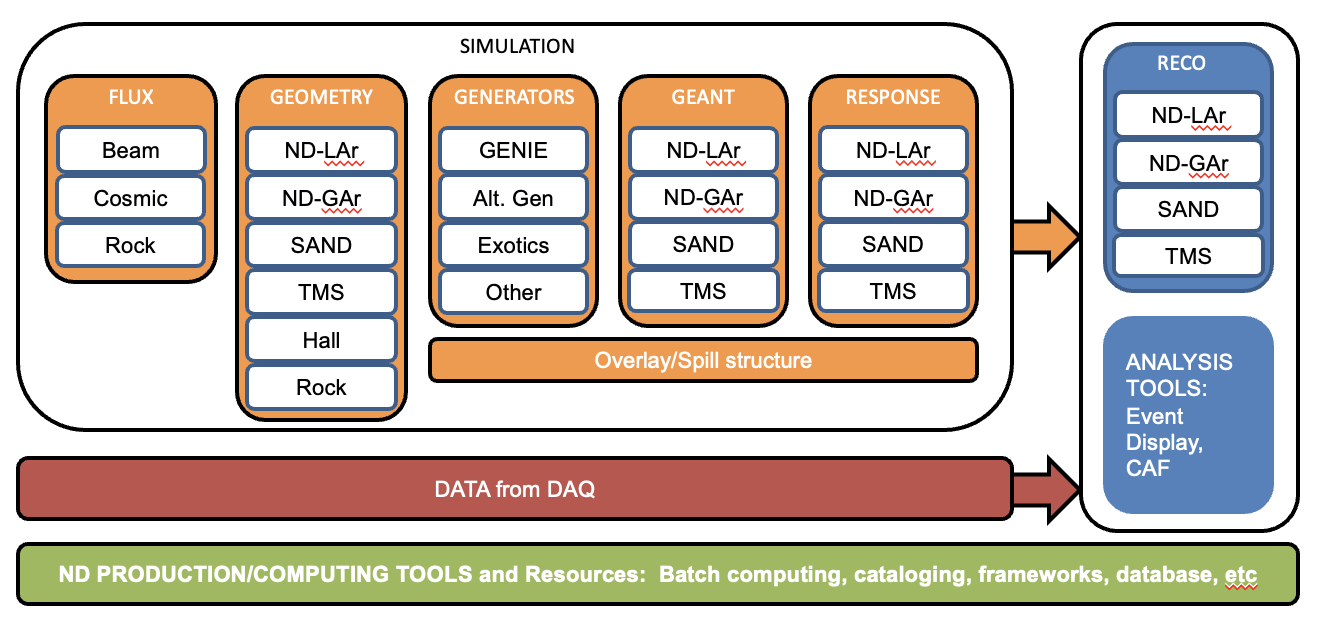
\includegraphics[width=0.8\textwidth]{graphics/Algo/ND_sim_reco_flowdiagram.png}
\end{dunefigure}

\subsection{Near Detector Response Simulation}

Each detector maintains it's own detector response simulation. 

\subsubsection{ND-LAr Detector Simulation}
\dword{ndlar} current has a integrated microphysical optical photon simulation and data-driven charge and pixel response model. 

\subsubsection{TMS Detector Simulation}
Current detector response is handled with general hit smearing. A full detector response simulation is in progress. 

\subsection{SAND Detector Simulation}
The SAND simulation software was developed to provide neutrino interaction samples in the SAND detector geometry, based on  GENIE+GEANT4 or FLUKA.The geometry includes a detailed description of the magnet, the yoke and the electromagnetic calorimeter and either the Straw Tube Tracker (STT) or 3D projection scintillator tracker plus (Time Projection Chambers 3DST+TPC) inner tracker. The calorimeter response is modeled  with energy and timing resolution based on results published by KLOE collaboration,
which had an excellent agreement between simulation and data.

\subsection{ND-GAr Detector Simulation}
\label{sec:usecases_ndgardetsim}

The \dword{garsoft} suite of \dword{art}-based modules is used to simulate the \dword{ndgar} detector.  It performs similar functions to \dword{larsoft}'s \dword{geant4} and detector simulation modules.  \dword{garsoft} includes interfaces to the following event generators:  \dword{genie}, CRY, and a text-file generator.  It also contains a \dword{larsoft}-like interface to \dword{geant4}, called {\tt garg4}.  In order to be used in conjunction with the other near detectors in a full hall simulation, \dword{garsoft} also includes a module to import energy deposits from {\tt edep-sim}, and format them internally as if they had been made by {\tt garg4}.

Once the energy deposits are available, a module that simulates the division between ionization and scintillation quanta is invoked.  Electron drift through the gaseous medium is parameterized, and longitudinal and transverse diffusion is modeled by sampling from Gaussian distributions of widths that grow with the square root of the drift time.  The effect of attenuation due to attachment of drifting electrons on electronegative impurities in the gas is also simulated at this time. 

The anode planes are modeled as re-purposed ALICE %inner and outer readout chambers (
\dwords{iroc} and \dwords{oroc} ~\cite{Dellacasa:2000bm}.  Charge is amplified by avalanches on the anode wires, and induced charge on the nearby readout pads provides the charge detection.  The pad response functions are taken from Ref.~\cite{Dellacasa:2000bm}.

The response of the calorimeter and the muon systems are parameterized versions of the energy deposit information, localized to the detector cells in which the energy is deposited.

\subsection{Overlays}
In order to build full beam spills simulated events on rock, detector fiducial volumes and the corresponding anti-fiducial sample are overlayed to reproduce expected beam timing and intensity. The OverlayGenie package is the current overlay tool in use but alternative which are more integrated are being developed. 


\section{ProtoDUNE Simulation Experience \hideme{Yang - draft}}

The \dword{fd}/\dword{protodune} \dword{larsoft}-based  detector simulation framework has already been tested successfully in \dword{protodune} and is described more fully in references \cite{DUNE:2021hwx,DUNE:2020cqd}.

The \dword{pdsp} simulation includes beam particles, cosmic ray interactions and radiological backgrounds. The beam particle species and momentum distributions are from the \dword{geant4} simulation of the H4-VLE beam line at CERN, which consists of $e^{+}$, $\pi^{+}$, $p$, and $K^{+}$ particles at 0.3, 0.5, 1, 2, 3, 6, and 7\,GeV/$c$. Cosmic ray interactions are produced with the Corsika generator. Radiological backgrounds, including $^{39}$Ar, $^{42}$Ar, $^{222}$Rn, and $^{85}$Kr, are also simulated using the RadioGen module in \dword{larsoft}. The primary particles are tracked in the \dword{lar} using the \dword{geant4} package. 
The ionization electrons are drifted towards the wire planes %anne. The  HMS agree
and the effects of recombination, attenuation and diffusion are simulated. The accumulation of positive ions in the detector modifies the trajectory of ionization electrons and the strength of the \efield, which is 
known as ``space charge effects''; this is simulated using the measured distortion and \efield maps. The electronic signal is simulated by convolving the number of electrons reaching each wire plane with the field response and electronics response. The field response is modeled using the \dword{garfield}\cite{Veenhof:1998tt} package. 
%done\todo{anne: I added the dword; add the definition please } 
The electronics response uses the parameterization from a \dword{spice} simulation with the average gain and shaping time measured in the \dword{protodune} charge injection system. 
%\hideme{cite the papers for protoDUNE}
%Each event corresponds to a 3 ms readout window with a sampling rate of 0.5$\mu$s per time tick.  The total number of electronic channels is 15,360. 
\section{General Simulation Considerations}

In addition to the specific needs for particular detectors there are additional common considerations for simulation. 

\subsection{Overlays or Mixing}
\label{sec:usecases_overlays}
An efficient method for accurately simulating backgrounds in high rate or high noise environments is to overlay the simulated interaction information on real data.  For example, the environment in \dword{protodune} or the near detector includes multiple beam and rock muon interactions in the same readout as %anne (made plural) an ok
the interactions of interest.  Libraries of properly formatted raw data can be combined with simulated hits from a simulated event to yield a realistic simulation of an interaction in the real detector. This requires a library of such interactions and careful matching of the running conditions of the external raw events to the desired simulated events. 

{\it Challenges: %We have 
DUNE has not yet integrated overlays into the \dword{protodune} or \dword{fd}  frameworks. %anne To do this we will need to 
Implementation of overlays will  require distribution of large volumes of overlay data to remote sites while maintaining randomness. Other experiments such as MicroBooNE and MINERvA have done this successfully. }

\subsection{Reweighting}
If intermediate simulation steps  are stored they can be used to reweight interactions to reflect new knowledge about the underlying cross sections, neutrino flux, detector materials or detector properties. Examples include the \dword{ppfx} beamline simulation reweighting system and the implementation of different cross section and final-state interaction models in event generators. 

{\it This is not a major challenge, several reweighting packages have been developed for NuMI/DUNE \cite{Aliaga:2015wva, Calcutt:2021zck}.}

\subsection{Outputs from Simulation}
%anne At this point we should have simulated data 
Once simulated data exists
that is equivalent to the raw data coming from the detector, %. The 
the next steps are calibration and reconstruction. In all cases, descriptive metadata needs to be produced that would allow reproduction of the simulation. 

{\it Possible challenge:  How many and which intermediate steps need to be stored permanently in order to optimize storage vs CPU utilization?}



\section{ProtoDUNE and Far Detector Reconstruction \hideme{Junk, Muether and Schellman-draft}}

%%%%%%%%%%%%%%%%%%%%%%%%%%%%%%%%


%\section{ProtoDUNEdata: raw data acquisition, cataloging and storage \hideme{Schellman - draft}}\label{sec:use:pdii-daq}



% \subsection{DAQ to Raw Data store \hideme{Schellman-draft}}
% The \dword{daq} and \dword{cisc} systems are expected to provide in close to real time:

% \begin{itemize}
%     \item Raw data from the \dword{tpc} and \dword{pd} detectors. 
%     \item Information on run and trigger configuration
%     \item Beam information
%     \item Information on detector conditions. For example, granular information on the \dword{hv} is needed to study and compensate for \dword{hv} fluctuations. 
%     \item Low level calibration constants such as gains that do not need extensive offline processing
    
% \end{itemize}


% The raw data are written to disk locally and then copied to the archive site (FNAL). Once the data are confirmed to be on tape, the local copy may be deleted.

% A second copy of the raw data will be stored in a different archive. 

% \subsection{Inputs to reconstruction}

% The run and trigger information, beamline  data, conditions and calibration constants are made available through separate data paths and stored in appropriate databases. In ProtoDUNE Run I, some of this information was transferred manually and stored in the \dword{sam} catalog.  DUNE document 22983 \cite{bib:docdb22983} describes the metadata strategy for ProtoDUNE II and DUNE. 

%Figure \ref{fig:ch:use:pdii} illustrates a typical reconstruction flow for ProtoDUNE data
\begin{dunefigure}
[Data flow diagram for standard ProtoDUNE reconstruction]
{fig:ch:use:pdii}
{Data flow diagram for standard \dword{protodune} data reconstruction. The central boxes show the processing steps, the right side shows the large-scale data flow,  and the left side shows the auxiliary information needed for processing. Thicker lines indicate particularly large data volumes.}
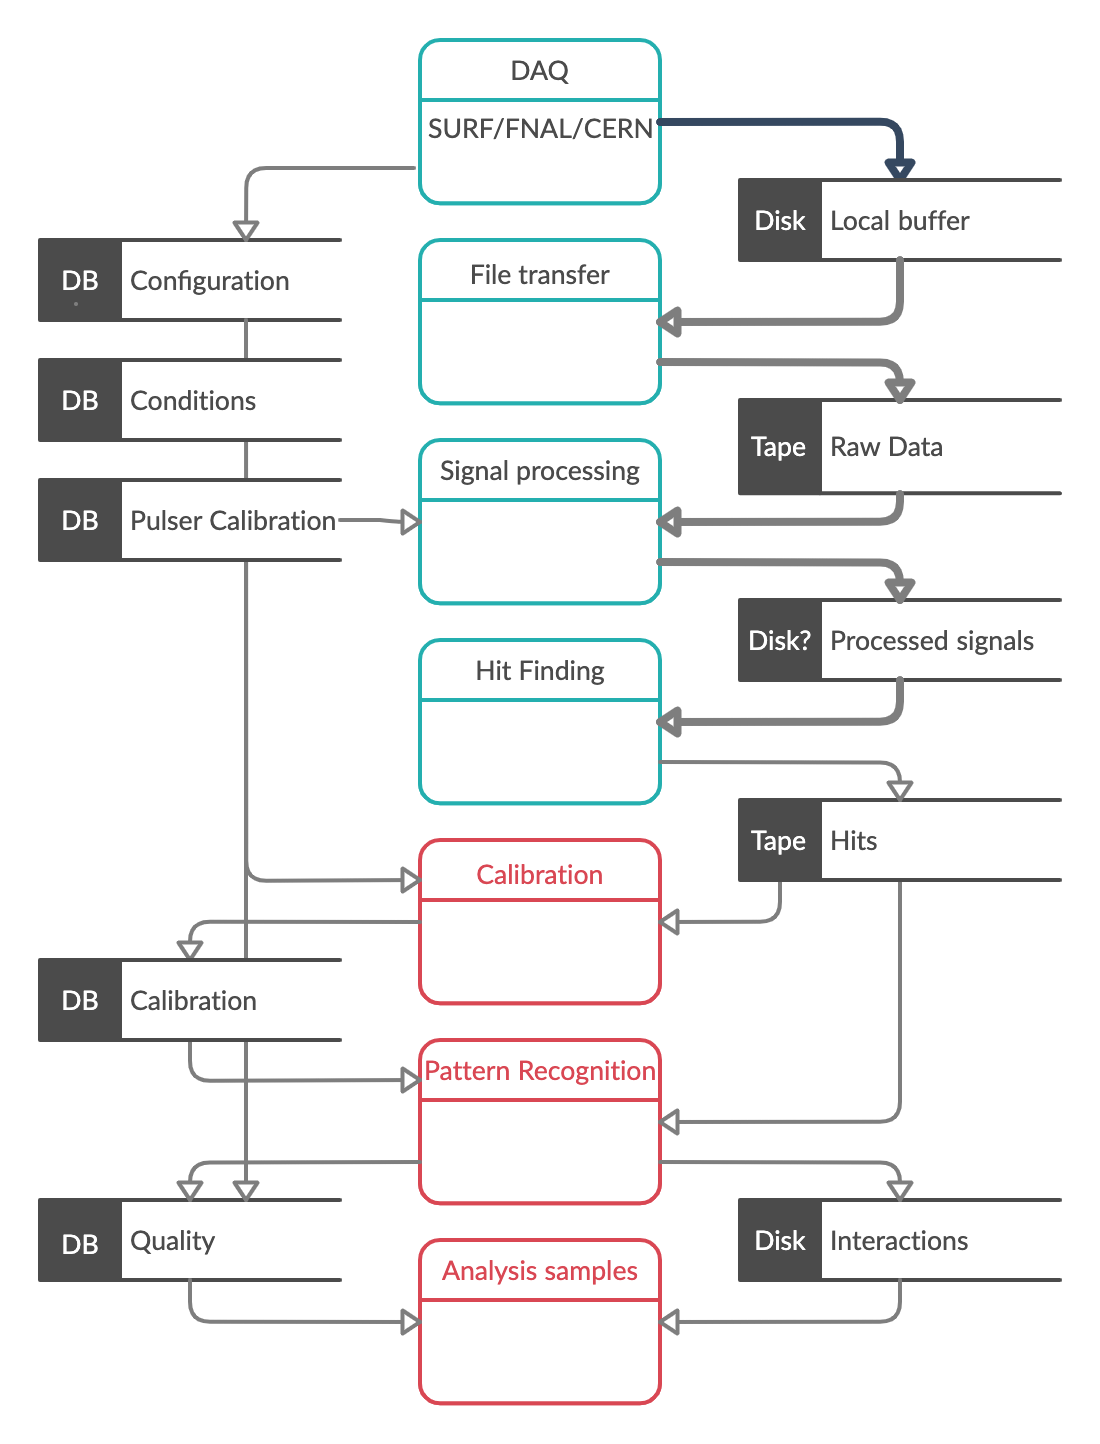
\includegraphics[width=0.8\textwidth]{graphics/IntroFigures/Data_processing_FD_v3.png}
\end{dunefigure}

%\subsection{ProtoDUNE and Far Detector Reconstruction\hideme{Schellman-draft}}\label{sec:use:pdii}

A detailed description of the \dword{pdsp} and Far Detector reconstruction algorithms is given in Ref.~\cite{DUNE:2020ypp}.  This section outlines those aspects of the reconstruction processing that are directly related to software and computing issues.
Figure~\ref{fig:ch:use:pdii} shows the data flow for regular reconstruction in \dword{protodune}.  
There are, in principle,  multiple stages in reconstruction that are each well suited to different computer architectures.  We expect the full \dword{fd} data processing to follow a similar path to that used by \dword{protodune}.  

Figure \ref{fig:ch:use:fdagg} illustrates  readout structures for full DUNE \dword{fd} modules.  A readout consists of a large number (up to 150) of   30\,MB \dword{apa} readouts and a number of smaller readout fragments.  These need to be processed and  recombined into a single readout record. 

\begin{dunefigure}
[Data aggregation diagram for FD]
{fig:ch:use:fdagg}
{Data aggregation cases for the far detector. The top case shows information for normal beam or calibration readouts. A single file of $\sim 10$\,GB size contains several complete \dword{tr} with their boundaries designated by the dashed lines.  \dword{tpc} \dword{apa}'s, \dwords{pd},  trigger primitives and a trigger  are recorded for each trigger readout.  In addition, a manifest, which describes the relations between the data, is stored either in the file or in external metadata.  The bottom case is a \dword{snb} readout, in which thousands of 5-10\,ms time slices must be read out over 100\,s.  The solid lines denote file boundaries. How data are ordered, by geographical position or by time,    is not  yet specified.}
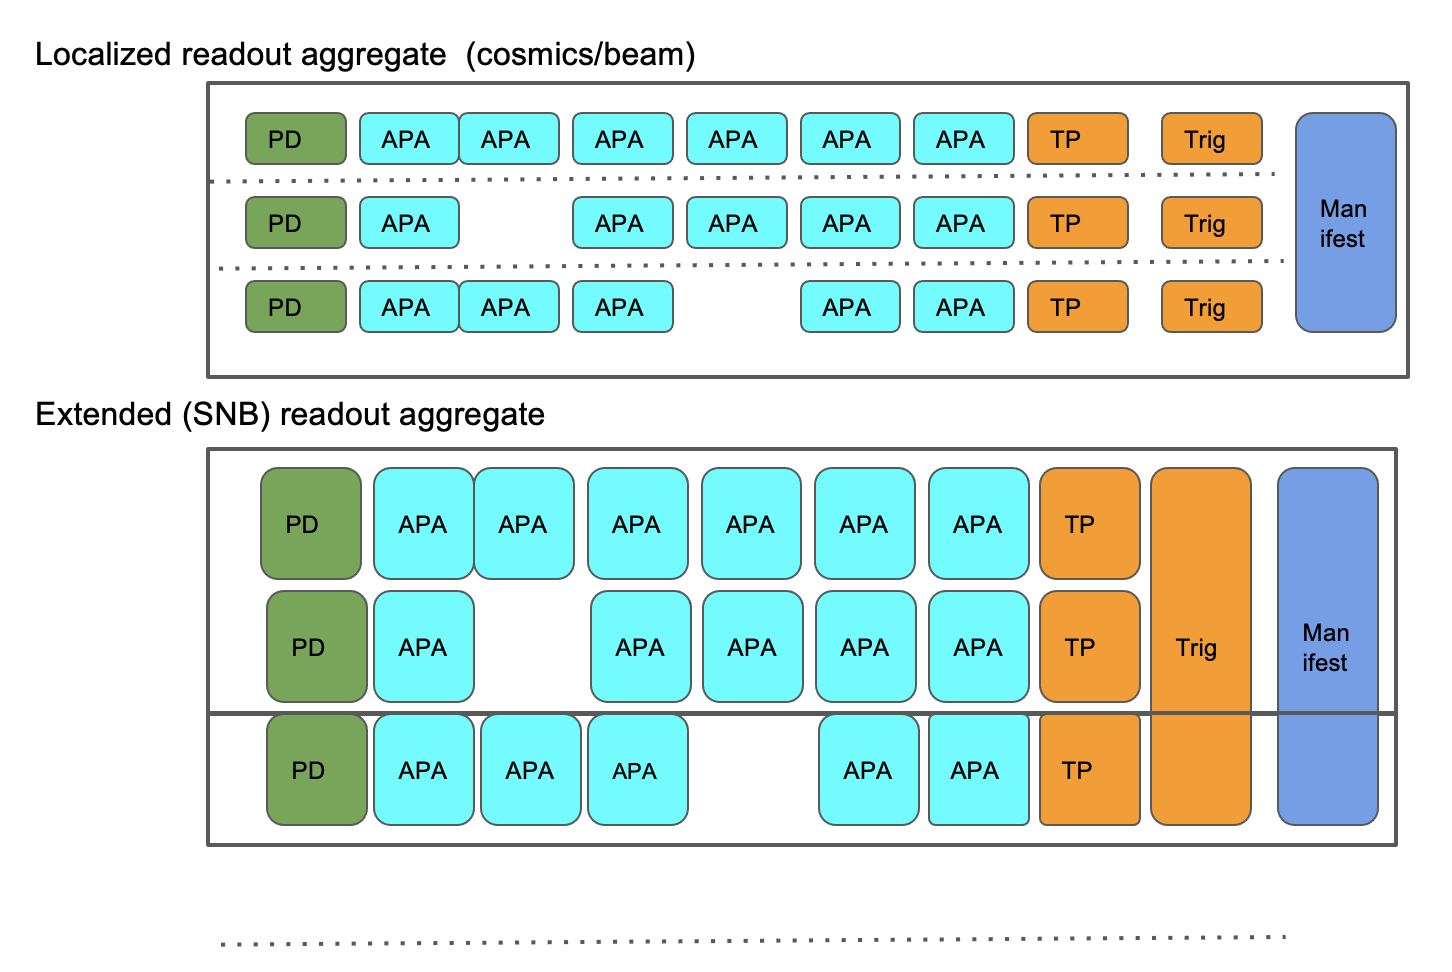
\includegraphics[width=0.8\textwidth]{graphics/IntroFigures/DataAggregation.png}
\end{dunefigure}
%\pagebreak

\subsection{Signal Processing \hideme{Schellman-draft}}

Reconstructing events in a \dword{lartpc} is challenging.  Each trigger record contains a large number of waveforms, one for each readout channel.  In \dword{pdsp}, the waveforms typically were 6000 time ticks long, with one \dword{adc} sample per time tick.  A detailed description of the reconstruction procedures, starting with these waveforms, is given in~\cite{Abi:2020mwi}, and summarized briefly here.


The signal processing step takes the raw waveforms, applies  basic channel-to-channel calibrations, removes noise and stuck bits, and performs 1D or \twod deconvolution.   In the \dword{tpc}, this processing step operates on large \twod data arrays and may be suitable for different architectures than conventional pattern recognition. For the \dword{pd}, 1D data arrays will be the input. It is anticipated that the signal processing step will not need to be done frequently. 

The input data at this point are quite uniform, effectively bit streams from \dword{tpc} and \dword{pd} channels.  There are correlations between channels in the \dword{tpc} data that require concurrent processing of multiple channels.  Segmentation at the level of a readout plane within an \dword{apa}  or \dword{lem} is desirable.  An uncompressed input \dword{apa} plane is of order 10\,MB of 12-bit words. 

%The output of this stage is still quite large even if lossless compression algorithms are applied. 


Typically, data from a single-phase \dword{lartpc} \dword{daq} are stored as compressed sequences of data frames, containing 128 or 256 channels worth of data on each time sample.  These must be decompressed and rearranged into sequences of \dword{adc} values corresponding to the original waveforms.  Additional decoder modules are run to unpack \dword{pds}, \dword{crt} trigger and timing \dword{daq} fragments.
From there, mitigations are applied to correct, as best as possible, known failures of the front-end electronics.  As yet, these are only needed for the TPC readout electronics.  

A particular failure mode in \dword{pdsp} is the sticky-code problem, which is mitigated by interpolating neighboring \dword{adc} samples in time.  Channel-to-channel gain corrections are applied, correlated noise is filtered out, the pedestal is found, and a correction is made for the \dword{ac} coupling between the preamp and the \dword{adc}.  The \dword{adc} mitigation, correlated noise removal, gain correction, pedestal finding and \dword{ac} coupling corrections are grouped into the data preparation module.  The \dword{wirecell} toolkit~\cite{wirecell,ref:wire_cell_toolkit,ref:pdune_signal_processing} provides a \twod deconvolution in wire index and charge arrival time, and it associates charge in the three views to produce a \threed image of the charge locations where it was produced.  

{\it Major challenge: The \dword{tpc} data need to be processed with a minimum granularity of a readout plane as multiple wires must be combined to achieve the best \twod deconvolution.  Each plane produces of order 10 million 12-bit samples/readout window. After decompression into 32 bit words, the input data size %anne/APA
per \dword{apa} is of order 30\,MB per plane. This phase of data processing is well suited to parallel processing on GPU's or \dwords{fpga} but imposes new requirements on the event reconstruction framework. }

\subsection{Hit Finding and Pattern Recognition}

The calibrated, filtered, deconvolved waveforms are then used as input to a hit-finding algorithm, which identifies peaks in the waveforms and fits Gaussians to each proposed peak.  These hits are then used as inputs to general reconstruction algorithms, such as the SpacePointSolver~\cite{DUNE:2020ypp} \dword{pandora}~\cite{Marshall:2015rfa}, TrajCluster~\cite{ref:trajcluster}, and \dword{pma}~\cite{ref:PMA}, which identify clusters, tracks and showers in \threed by associating objects in the three \twod views.  The calorimetry modules sum up and calibrate the charge deposits for use in energy reconstruction and \dword{pid}.  The parameters of the clusters, tracks and showers are stored in \dword{root} trees that end users can analyze rapidly and repeatedly.

Additional modules find hits in the \dword{pd} waveforms and group them into clusters called flashes.  The \dword{crt} data are analyzed in dedicated modules that produce associations between hits in the upstream and downstream \dword{crt} modules for use in analyses.

Separating track-like energy deposits from shower-like deposits is a key part of many DUNE analyses.  This is accomplished with a \dword{cvn} called {\tt EmTrackMichelID} in Table~\ref{tab:protodune_cpu_reco_by_module}.  It is one of the most CPU-intensive operations in the \dword{pdsp} reconstruction chain, when the algorithm is run on a grid node lacking a GPU.  Recently, however, a \dword{gpuaas} technique has been developed~\cite{Wang:2020fjr}, enabling a speed-up on the order of a factor of ten, though it depends on the ratio of CPU-only nodes to GPU resources.


\subsection{ProtoDUNE Experience\todo{Schellman/Yang, ok 3/13}}

\begin{longtable}
{l r}
\caption[Processing time for reconstruction modules for a \dword{pdsp} event]{Wall-clock module execution times for the reconstruction of a typical \dword{pdsp} event, in seconds.  Processes taking less than 1 second are not shown. The event is a data event from Run 5809, a 1\,GeV beam run.
Note that the electromagnetic shower reconstruction module EmTrackMichelId  dominates. } \\ \toprowrule
  \rowcolor{dunesky}
Module Label & time/event (sec)\\ \toprowrule
RootInput(read)                          &     0.14\\%7283          \\
%timingrawdecoder:TimingRawDecoder        &     0.0095498         \\
%ssprawdecoder:SSPRawDecoder              &     0.126099          \\
%crtrawdecoder:CRTRawDecoder              &     0.0181903         \\
%ctbrawdecoder:PDSPCTBRawDecoder          &     0.0204753         \\
beamevent:BeamEvent                      &      1.6\\%54           \\
caldata:DataPrepByApaModule              &      83.0\\%24          \\
wclsdatasp:WireCellToolkit               &      79.9\\%16          \\
gaushit:GausHitFinder                    &      1.6\\%342          \\
%nhitsfilter:NumberOfHitsFilter           &    0.00177549         \\
reco3d:SpacePointSolver                  &      9.4\\%157          \\
hitpdune:DisambigFromSpacePoints         &      1.5\\%541          \\
pandora:StandardPandora                  &      39.9\\%87          \\
%pandoraWriter:StandardPandora            &     0.370009          \\
pandoraTrack:LArPandoraTrackCreation     &      4.6\\%221          \\
pandoraShower:LArPandoraShowerCreation   &      3.7\\%432          \\
pandoracalo:Calorimetry                  &      2.1\\%152          \\
pandoracalonosce:Calorimetry             &      1.9\\%852          \\
%pandorapid:Chi2ParticleID                &     0.0115046         \\
%pandoracali:CalibrationdEdXPDSP          &     0.106919          \\
%pandoracalipid:Chi2ParticleID            &    0.00851985         \\
pandoraShowercalo:ShowerCalorimetry      &      3.3\\%953          \\
pandoraShowercalonosce:ShowerCalorimetry &      3.2\\%698          \\
emtrkmichelid:EmTrackMichelId            &      233.8\\%4          \\
%ophitInternal:OpHitFinder                &     0.0190084         \\
%ophitExternal:OpHitFinder                &    0.00828164         \\
%opflashInternal:OpFlashFinder            &     0.0172739         \\
%opflashExternal:OpFlashFinder            &    0.000597182        \\
%opslicerInternal:OpSlicer                &     0.0184422         \\
%opslicerExternal:OpSlicer                &    0.00538796         \\
%crttag:SingleCRTMatchingProducer         &     0.0231673         \\
c%rtreco:TwoCRTMatchingProducer           &     0.0128138         \\
anodepiercerst0:T0RecoAnodePiercers      &      1.1\\%673          \\
pandora2Track:LArPandoraTrackCreation    &      11.6\\%25          \\
pandora2calo:Calorimetry                 &      4.9\\%932          \\
pandora2calonosce:Calorimetry            &      4.5\\%118          \\
%pandora2pid:Chi2ParticleID               &     0.0211641         \\
%pandora2cali:CalibrationdEdXPDSP         &     0.0867829         \\
%pandora2calipid:Chi2ParticleID           &     0.0206842         \\
pandora2Shower:LArPandoraShowerCreation  &      4.2\\%815          \\
pandora2Showercalo:ShowerCalorimetry     &      4.2\\%29           \\
pandora2Showercalonosce:ShowerCalorimetry&      3.8\\%562          \\
%TriggerResults:TriggerResultInserter     &     0.000349372        \\
%RootOutput                               &    2.8912e-05         \\
RootOutput(write)                        &     2.8\\%458               \\
{\bf Total:}                             &     {\bf 507.9}      \\ \colhline
\label{tab:protodune_cpu_reco_by_module}
\end{longtable}


%\subsection{Hit finding}
%The processes signal information is then searched  for groups of  channels above threshold and fit to Gaussian pulses shapes.  This step is computationally quite different from the signal processing phase as it involves searching and fitting. 
%
%The outputs are Gaussian fits to the pulses. This output is substantially smaller than the processed hit information. 
%
%{\it The major challenge here is the radically different processing modality relative to hit finding.  Where signal processing can largely be implemented by matrix operations, hit finding algorithms make heavy use of code branching and external fitting algorithms. Accommodating both signal processing and hit finding on a single  architecture may be challenging. }

\section{Near Detector Reconstruction\hideme{Junk/Muether - needs revision}}

The \dword{nd} Reconstruction primary exists as separate reconstructions for each individual ND sub-detector (described below). The ND software group are developing a common data model which will allow inter-detector software connection. For instance, an event matching algorithm between the \dword{ndlar} and TMS has been developed. Output from the Reconstruction will be written to common analysis files (CAF) that will enable physics analysis (Fig. \ref{fig:nd:reco}). The current ND data model is outlined in the DUNE ND Data Model document~\cite{bib:docdb24735}.

\begin{dunefigure}
[ND Reconstruction Flow Chart Example]
{fig:nd:reco}
{An example ND Reconstruction WorkFlow is shown for simulation with TMS and LAr (MLReco) data producing track matching information and stored in CAF.}
{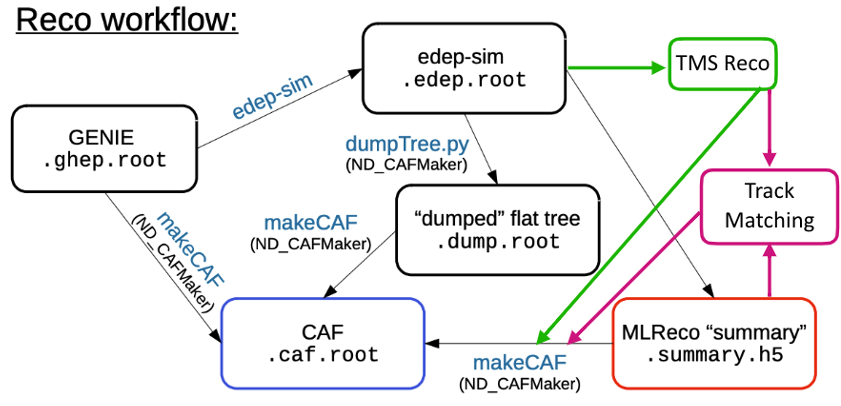
\includegraphics[width=0.8\textwidth]{graphics/ND/ND-Reco-workflow.png}}
\end{dunefigure}

\subsection{LAR}
 Reconstruction algorithms for the \dword{ndlar} include both traditional and machine learning-based chains. The primary reconstruction is an automated machine-learning based package which has been demonstrated on full spill events on in native 3d detector readout. A parallel Pandora based reconstruction is also being prepared. These reconstruction algorithms are currently being tested on both simulated and prototype data. 

\subsection{TMS}
The output of the \dword{tms} reconstruction will inform the \dword{ndlar} reconstruction as to which tracks exited the \dword{ndlar} and were reconstructed in the \dword{tms}. A stand-alone \dword{tms}-reconstruction also enables monitoring of the inclusive neutrino event rate, using neutrinos interacting on the \dword{tms} fiducial volume.

The current \dword{tms} reconstruction approach is running the track finding and reconstruction simultaneously through a Kalman filter, or having a separate track finding algorithm identify track candidates which it feeds to the Kalman track reconstruction.

\subsection{Track finding}
For the track finding stage, we are currently investigating three approaches. They all run in each view separately, and the 2D to 3D track matching and merging is done at a later stage.

\begin{itemize}
    \item Perform a Hough transform \cite{hough} in each view separately, and find which hits intersect the primary Hough line. Traverse the hits and group neighbouring hits into a track candidate. Take remaining hits (not belonging to a candidate) and repeat process to see if there is a $N^{th}$ track candidate. Due to the bending in the $x-z$ view, the Hough transform is often more successful in the $y-z$ view, and the neighbour clustering in $x-z$ is critically important.

    \item Sort the hits in $z$, and run a custom A* path finding algorithm from first to last hit in $z$. The intent is to find the shortest path between the first and last hit, only traversing cells that have been hit. If no path is found from start to finish, repeat A* path finding running until the hit with second largest z, and continue.
    
    \item Sort the hits in $z$, and run a Kalman filter from first to last hit in $z$. For this to succeed, the Kalman filter needs to account for the energy-loss, bending and multiple-scattering happening in the iron and scintillator layers. 
\end{itemize}

\subsection{Track reconstruction}
Currently, the lepton candidate is assumed to be the longest track in the track finding. After the reconstruction stage, it is envisioned the lepton candidate is assumed to be the most energetic track that fits a muon hypothesis. Depending on the final design of the \dword{tms}, the track reconstruction will operate on 2D or be combined into 3D views. 

Preliminary studies show track length is by far the most important feature for a good muon KE measurement, with the energy deposits and track bending being secondary contributions. The current Kalman implementation in the \dword{tms} software includes effects from energy loss and multiple scattering, inspired by similar implementations in \dword{minos}, \dword{minerva}, and \dword{t2k}. Efforts towards integration of the \dword{ndlar} and \dword{tms} reconstructions are also ongoing.

\subsection{Pixel-Based Gaseous Argon TPC Recontruction}
\label{sec:algo:reco:gartpc:pixels}

The \dword{ndgar} consists of two primary detectors -- a copy of the ALICE pixel-based \dword{tpc} in a 10-bar gas consisting predominantly of argon, surrounded by a calorimeter and a superconducting magnetic coil.  A muon system is envisaged outside of the calorimeter but is not included in the simulation or the reconstruction at the time of writing.  Data are unpacked and hits are found on the per-readout-pad waveforms, similarly to how the initial stages of reconstruction for a \dword{lartpc} are followed.  Hits are then clustered into TPC clusters, which reduces the memory and CPU usage of subsequent steps, and also increases the spatial resolution of individual clusters.  Vector hits are found by grouping TPC clusters into short line segments, and the vector hits themselves are grouped into track candidates by a pattern recognition module.  A track fit based on a Kalman filter then finds the best estimates of the track parameters.  Vertices are then found using tracks with nearby endpoints.  Because there is a cathode in the middle of the drift volume in the nominal \dword{ndgar} design, 
a cathode stitch module is then run to associate track segments on either side of the cathode, bring them together by solving for the best interaction time that lines the segments up, and also moves the associated tracks and vertices.  Vees ($K^0_s$ and
$\Lambda^0$ candidates) are found by pairing nearby tracks together, optionally requiring a displacement from another vertex, and forming the invariant mass.  The calorimeter consists of a mixture of strips and pads.  Calorimeter hits are found in the \dword{sipm} waveforms provided by the calorimeter \dword{daq}, and they are clustered together to form reconstructed three-dimensional energy deposit objects with positions, directions, and energies.  Calorimeter clusters are associated with tracks, and they must match both in position and in time.  Before association with a calorimeter cluster, a track's position along the drift direction is uncertain due to the unknown interaction time.
The nanosecond-scale timing resolution of the calorimeter allows the updating of track positions along the drift direction.

\subsection{SAND}

A preliminary full reconstruction of the events has been developed and includes identification of the primary charged particles and determination of the vertex position and momentum . For neutrons, identified as isolated clusters, techniques have been developed for distinguishing between primary and secondary neutrons and for primary particles the energy is reconstructed by the time of flight between the vertex and the cluster signal. Additionally, momentum and energy for neutral pions are obtained by the signal of daughter photons detected in the calorimeter or inside the tracker.
The software is at a preliminary stage and development continues on final reconstruction of primary particles detected in different sub-detectors and for identifying external neutrino interactions and background events.

\subsection{Common ND analysis files}

The final output format used to conduct physics analysis will be a simplified
{\it analysis tree} file, which contains a reduced subset of the full simulation
and reconstruction output. The first version of the analysis tree format is
based on the ND CAFs, which are produced by applying a parametric response
model to the Geant4-level ND simulation for use in long-baseline and other analyses.

\begin{dunetable}
[Average \dshort{ndgar} event wall-clock module execution times]
{l r}
{tab:garsoft_cpu_reco_by_module}
{Average wall-clock processing time for reconstruction modules for \dword{garsoft} events consisting of just one interaction in the gas.  An actual spill will contain of order 60 interactions, mostly  in the calorimeter, though many tracks will pass through the gas.}
Module Label & time/event (sec)\\ \toprowrule
RootInput(read)                             &    0.00\\%0353765       \\
init:EventInit                         &    1.31275e-05       \\
hit:CompressedHitFinder                &    0.00488308        \\
tpcclusterpass1:TPCHitCluster          &     0.0091922        \\
vechit:tpcvechitfinder2                &     0.0103787        \\
patrec:tpcpatrec2                      &     0.0130245        \\
trackpass1:tpctrackfit2                &     0.014211         \\
vertexpass1:vertexfinder1              &    0.000851081       \\
tpccluster:tpccathodestitch            &     0.0269436        \\
track:tpctrackfit2                     &     0.0135842        \\
vertex:vertexfinder1                   &    6.19847e-05       \\
veefinder1:veefinder1                  &    9.96417e-05       \\
sipmhit:SiPMHitFinder                  &    0.00153375        \\
sscalohit:CaloStripSplitter            &     0.0547754        \\
calocluster:CaloClustering             &    0.00492599        \\
trkecalassn:TPCECALAssociation         &    0.000237503       \\
TriggerResults:TriggerResultInserter        &    2.36397e-05       \\
RootOutput                                  &    3.6783e-06        \\
RootOutput(write)                           &    0.214077         \\
{\bf Total}                                  &     {\bf 0.369802}       \\ 
\end{dunetable}


\section{Calibration \hideme{Schellman-draft}}

Before final pattern recognition can be applied to physics events,  the processed hits from calibration samples (subsets of the full data, sometimes with special conditions) are run through specialized pattern recognition and used to derive high-quality calibration constants which are stored in the conditions database for future use.  Inputs include processed hit data but also detailed information about the configuration of the calibration system.  This step will likely be done many times, especially at the start of the experiment. Calibration samples may be taken quickly and may be very large, for example 500\,TB for a full laser calibration of the far detector. They will require occasional fast processing of PB-scale data samples. 

{\it Major challenge: The large size of some calibration samples means that fast processing for monitoring and fast application will require peaks in data storage and processing at rates considerably higher than normal data taking.}

%\subsection{Hits to reconstructed interactions }
%In this step, the improved calibration constants and raw hits are input to the full  pattern recognition and reconstructed interactions are output. Data quality can be monitored as part of this processing and stored. 
%
%Here a wide range of algorithms may be used. 
%
%{\it Challenge:  At some point after either signal or  hit processing, the data from a full interaction must be brought together in memory in an appropriate format for pattern recognition. Each \dword{apa} can still produce up to 1 MB of hits, leading to memory footprints of up to 100 MB for pattern recognition inputs.}

\section{Visualization}
\label{sec:visualization}
%anne starting to look at this 3/2
Both raw and reconstructed data from each of DUNE's detectors must be visualized graphically in multiple ways in order to successfully design, commission and operate the detectors, and to extract meaningful physics results.  While reconstruction is automated and hand-scanning is no longer used to extract physics results, event displays are critical for a large number of necessary steps:
\begin{enumerate}
    \item {\bf Design of the detectors}   It is important to visualize interactions in the detectors in order to ascertain which among them are easy to identify and measure, and which ones are difficult.
    \item{\bf Optimizing reconstruction algorithms}  Comparisons of true particle trajectories and energies with reconstructed versions thereof in simulated interactions provides guidance for improving reconstruction algorithms.  Quantitative metrics such as completeness and purity can be optimized, but it is easier to do so when viewing an event display that shows which pieces of which interactions have failed to reconstruct well.
    \item{\bf Operating prototypes and learning from them}  Data from prototypes, such as the \dwords{coldbox}, the \dwords{protodune}, and \dword{iceberg} must be analyzed quickly to ascertain what the noise level is and to search for the presence of signals.  This is part of an iterative experimental process to commission the prototypes by searching for noise sources, checking \dword{hv} and cryogenic performance, drift medium purity, etc.  Dead channels or other artifacts such as long-range induction effects are plainly visible on raw data displays.  Various artifacts may be addressable with software, such as correcting for front-end amplifier artifacts, correlated noise, and \dword{adc} issues.  These are all discovered first with event visualization.
    \item{\bf Interpreting calibration data}  Laser calibrations, neutron source data and radioactive source data must be inspected first before use, as unanticipated artifacts may confound the intended calibration use.
    \item{\bf Providing educational and public outreach materials}  Introducing new students to DUNE's physics program involves showing them what interactions look like in each of our detectors.  Materials for DUNEs public-facing web sites and press releases also require high-quality data visualizations.
\end{enumerate}
Each of these uses places different requirements on the visualization software.  Furthermore, the event display programs must be responsive and easy to use, though specialist functions may require additional configuration.

\subsection{Two-Dimensional Event Displays}
\label{sec:visualization:2d}

The data from the \dword{sphd} and \dword{spvd} modules are inherently two dimensional, with \dword{adc} values read out per wire (or strip) for each sample time.  Inspecting the raw waveforms side by side in a grayscale or colored map for each of the three views is critical for understanding the features of the raw data.  \dword{larsoft} provides such a display,
optimized for X-Window connections.  Users can zoom in on rectangular subsets of the data and clicking on the image brings up a one-dimensional waveform plot for the corresponding channel.  An example of such a display for a \dword{pdsp} event with cosmic rays is given in Figure~\ref{fig:vis:larsoftraw}.  An example of a two-dimensional display of reconstructed tracks, vertices and showers is given in Figure~\ref{fig:vis:larsoftreco}.  

\begin{dunefigure}
[LArSoft Raw Data Display]
{fig:vis:larsoftraw} 
{Example raw data display produced with \dword{larsoft}.  One \dword{apa}'s worth of data are shown for a \dword{pdsp} trigger record. The top panel shows the collection-plane data, the next panel V-plane data, and the bottom colored panel shows U-plane data.  Below those three is a single channel's waveform.  The colored panels show the pedestal-subtracted \dword{adc} values for each channel on the horizontal axes with sample time in 500~ns ticks on the vertical axes.  The time between samples is 500\,ns.  White vertical lines in the collection plane correspond to channels that have been flagged as noisy or dead.}
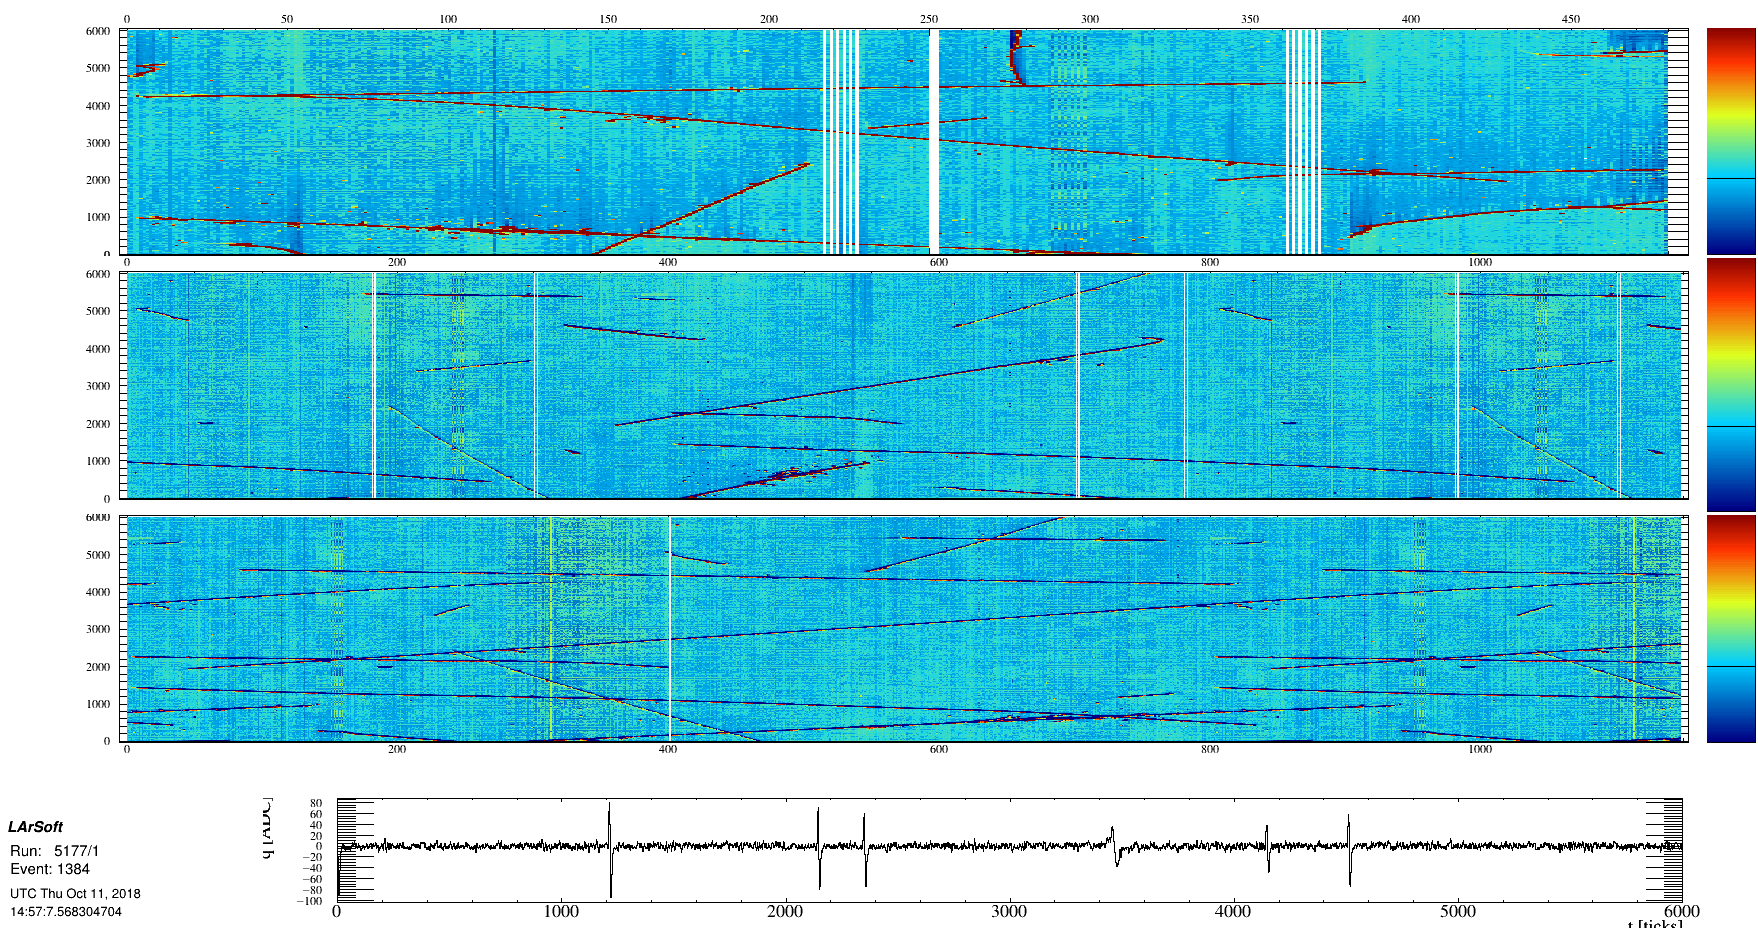
\includegraphics[width=0.9 \textwidth]{graphics/EventDisplays/pdsp_larsoft_rawevent.png}
\end{dunefigure}

The raw data display provided by \dword{larsoft} is best run interactively.  The user can step through the events in a file, forwards or backwards, or skip to a desired event number.  This event display is not built for non-interactive use.  There are use cases in which large numbers of raw event displays need to be produced in a batch.  For this purpose, dedicated modules have been written in DUNE's \dword{larsoft}-based software that provide two-dimensional displays of raw data and data that have been processed through each step of data preparation. Examples are shown in Figure~\ref{fig:vis:dataprep} after four stages of data processing.


\begin{dunefigure}[Two-Dimensional Displays of ProtoDUNE-SP Data in Stages of Data Preparation]{fig:vis:dataprep}{Example batch-mode event displays for a collection plane showing background reduction in successive stages of data processing.
For each plot, the horizontal axis is the readout sample time in 500~ns ticks, and the vertical axis is the channel number.
The color scale represents the charge for each channel averaged over five ticks
with the range chosen to make the noise visible.
Signals from charged tracks appear mostly in black and are off scale, well
above the noise level.  From Ref.~\cite{DUNE:2020cqd}}
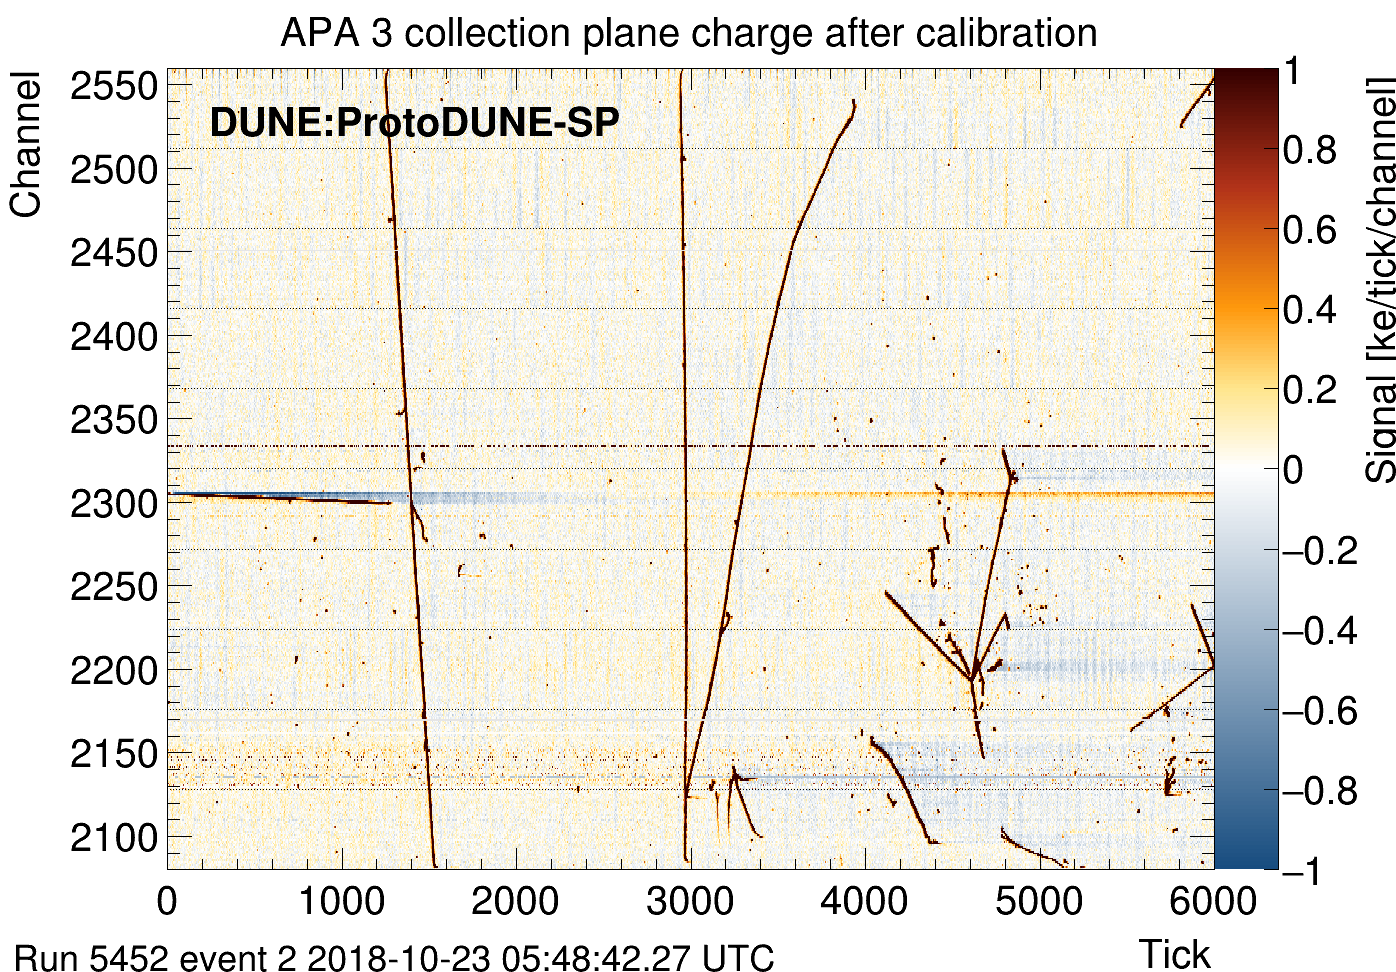
\includegraphics[width=0.49\textwidth]{graphics/EventDisplays/adccal_tpp0z_run005452_evt000002.png}
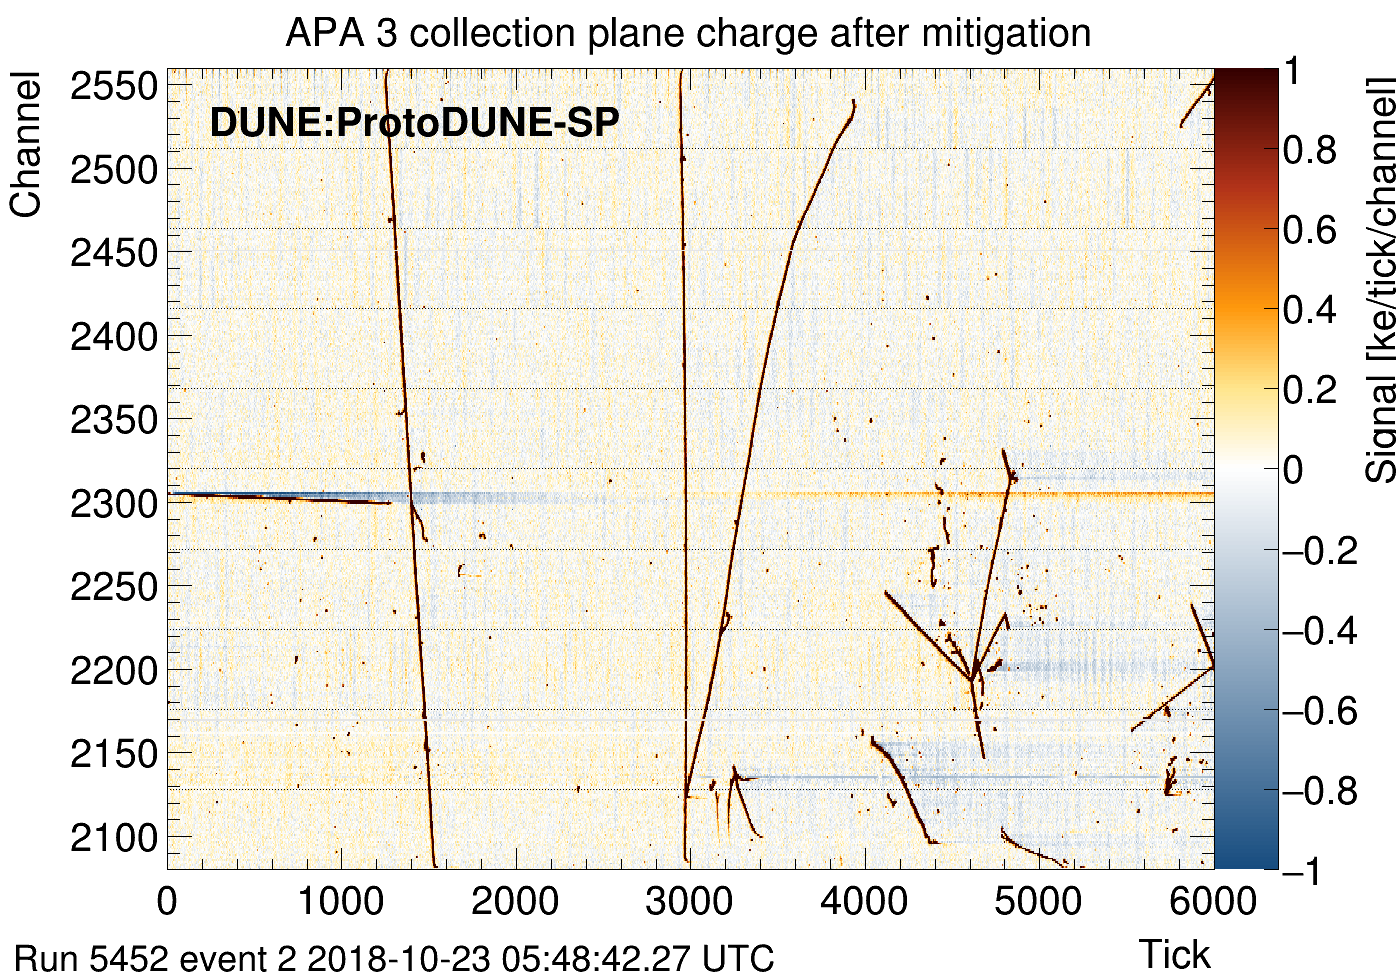
\includegraphics[width=0.49\textwidth]{graphics/EventDisplays/adcmit_tpp0z_run005452_evt000002.png}
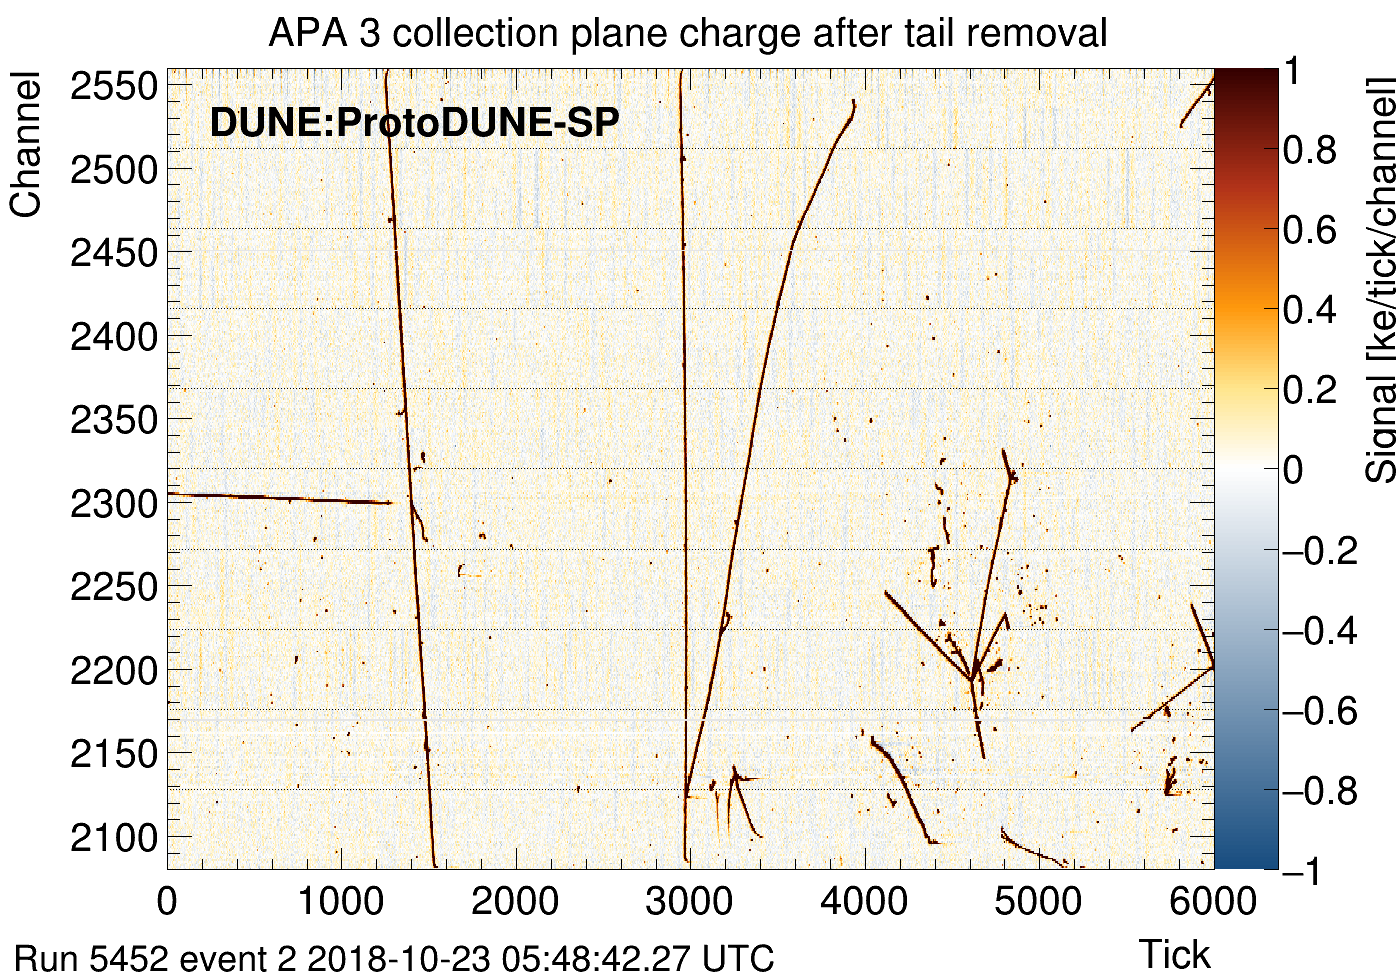
\includegraphics[width=0.49\textwidth]{graphics/EventDisplays/adctai_tpp0z_run005452_evt000002.png}
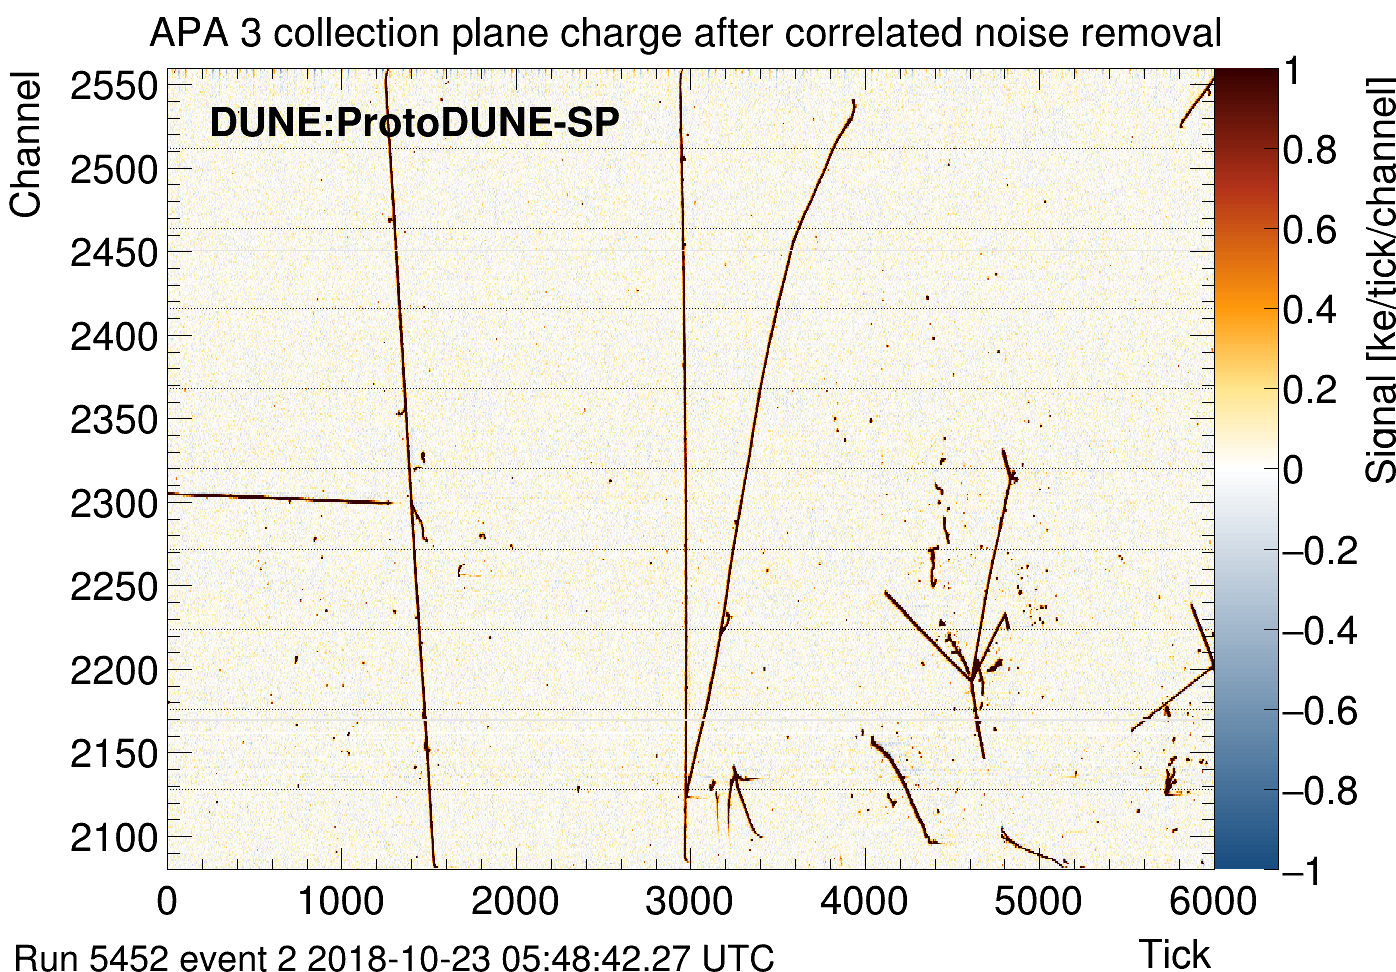
\includegraphics[width=0.49\textwidth]{graphics/EventDisplays/adccnr_tpp0z_run005452_evt000002.png}
%\caption{After pedestal subtraction and calibration.}
%\caption{After ADC sticky code and timing mitigation.}
%\caption{After tail removal.}
%\caption{After correlated noise removal.}
\end{dunefigure}


\begin{dunefigure}
[LArSoft Reconstructed Data Display]
{fig:vis:larsoftreco} 
{Example reconstructed data display produced with \dword{larsoft}.  One \dword{apa}'s worth of data are shown for a \dword{pdsp} trigger record. The top panel shows the collection-plane data, the next panel V-plane data, and the bottom colored panel shows U-plane data.  Below those three is a single channel's deconvolved waveform and fitted hits.  Reconstructed vertices, tracks and showers are displayed in the top three panels, with identifying numbers attached to each.}
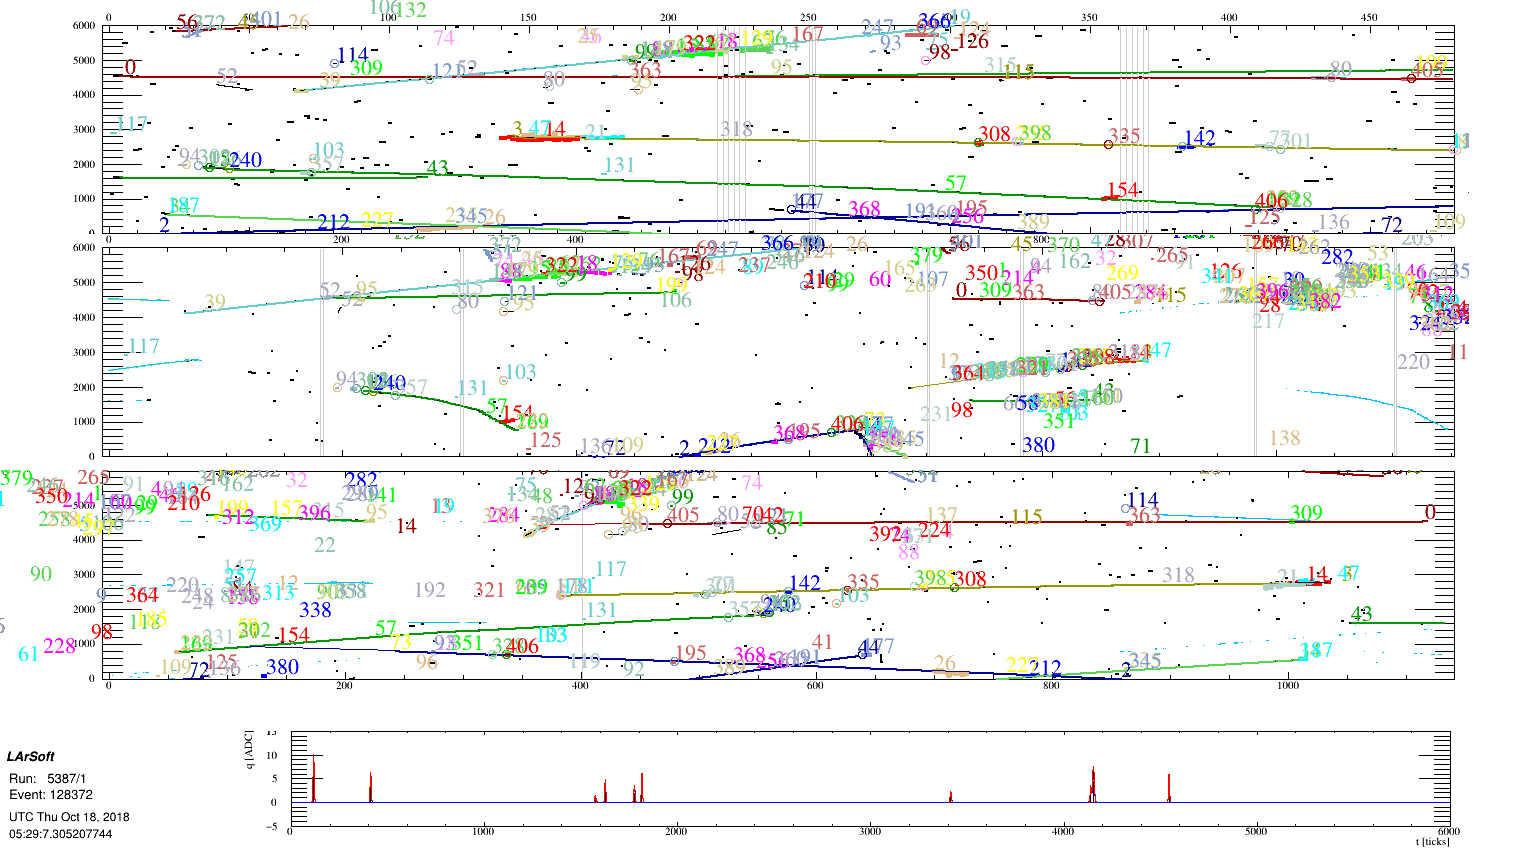
\includegraphics[width=0.9 \textwidth]{graphics/EventDisplays/larsoft_reco_example_evd.png}
\end{dunefigure}

%this event is the first one in this file:  np04_raw_run005387_0080_dl11_reco1_38694915_0_20201116T180838Z_reco2_48964460_0_20210930T150928Z.root

\subsection{Three-Dimensional Event Displays}
\label{sec:visualization:3d}

 LArSoft also provides a three-dimensional event display, showing the same reconstructed objects.  An example is given in Figure~\ref{fig:vis:larsoft3dreco}.  Only reconstructed objects are available in three dimensions as the data in the ProtoDUNEs and the Far Detector modules are two-dimensional.
 
\begin{dunefigure}
[Three-dimensional LArSoft Reconstructed Data Display]
{fig:vis:larsoft3dreco} 
{Example three-dimensional reconstructed data display produced with \dword{larsoft}, showing data from a \dword{pdsp} trigger record, for all \dwords{apa}.  Reconstructed space points are shown in gray while shower cones are drawn in red.  The display can be pan, zoom, and rotate under user control.  The \dword{larsoft} \threed event viewer can also produce animated gifs.}
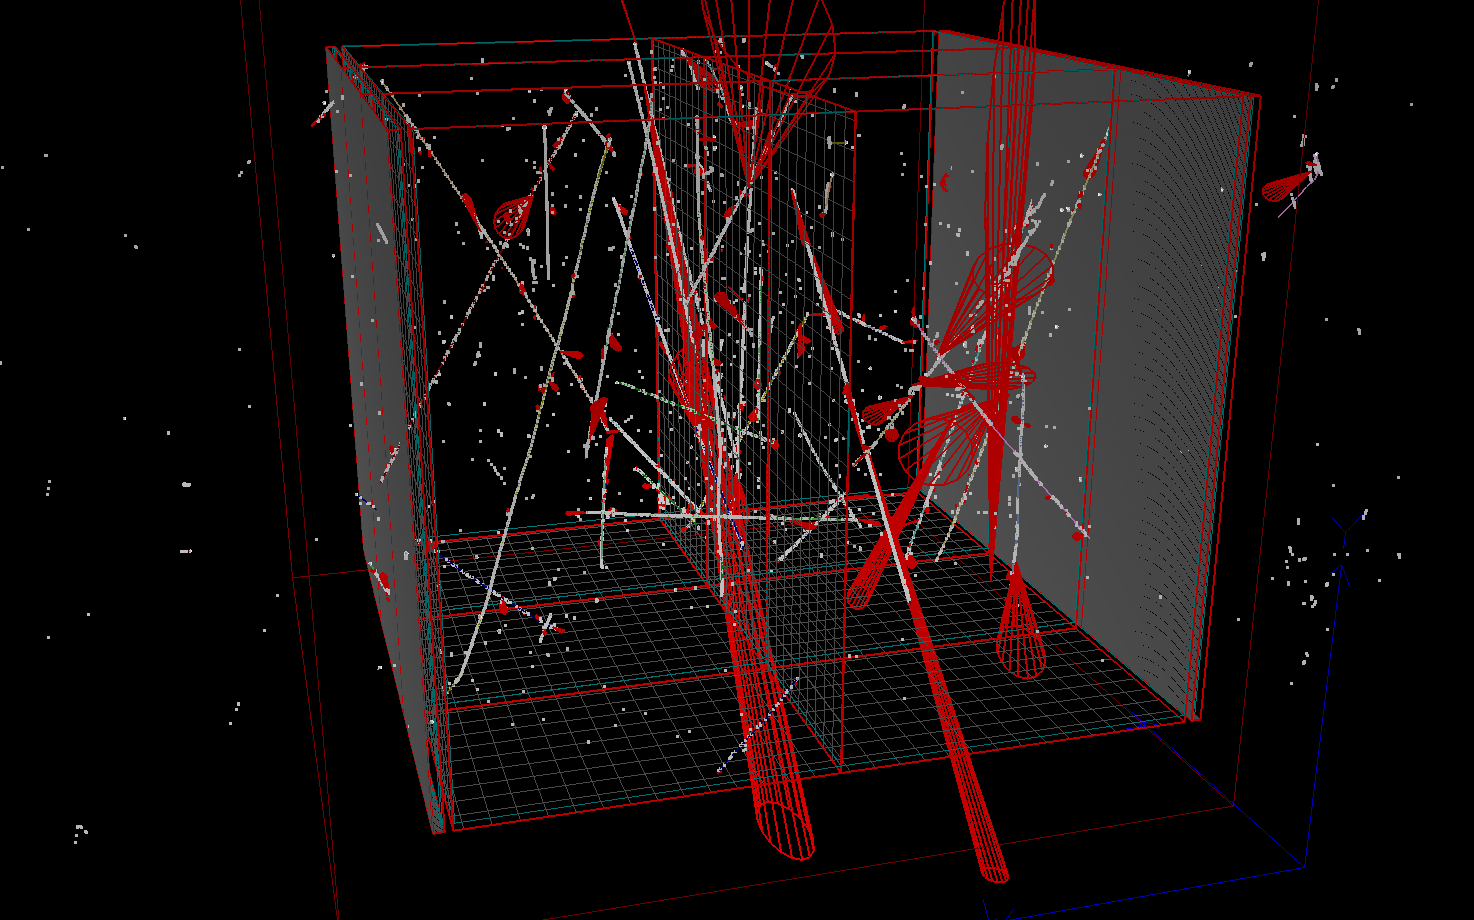
\includegraphics[width=0.8 \textwidth]{graphics/EventDisplays/larsoft_reco_evd_3d.png}
\end{dunefigure}

\subsection{Web-Based Event Displays}
\label{sec:visualization:web}

In addition to the \dword{larsoft}-based event displays, DUNE has multiple web-based event displays.  One, called the Bee event display, is made for displaying \dword{pdsp} events in a web browser.  The server is hosted at Brookhaven National Laboratory and contains a short list of typical \dword{pdsp} events, one of which is shown in Figure~\ref{fig:vis:bee}. No software needs to be installed on the user's computer, and no data files need to be copied.  The user only needs a modern web browser and the experience is enhanced with a capable graphics card.

\begin{dunefigure}
[Three-dimensional ProtoDUNE-SP Bee Data Display]
{fig:vis:bee} 
{Example three-dimensional reconstructed data display for a \dword{pdsp} data trigger record produced with the web-based Bee event display.  Users interact with the data needing only a modern web browser on their computer.  They can pan, zoom, rotate, and change display colors, point sizes, and transparency.}
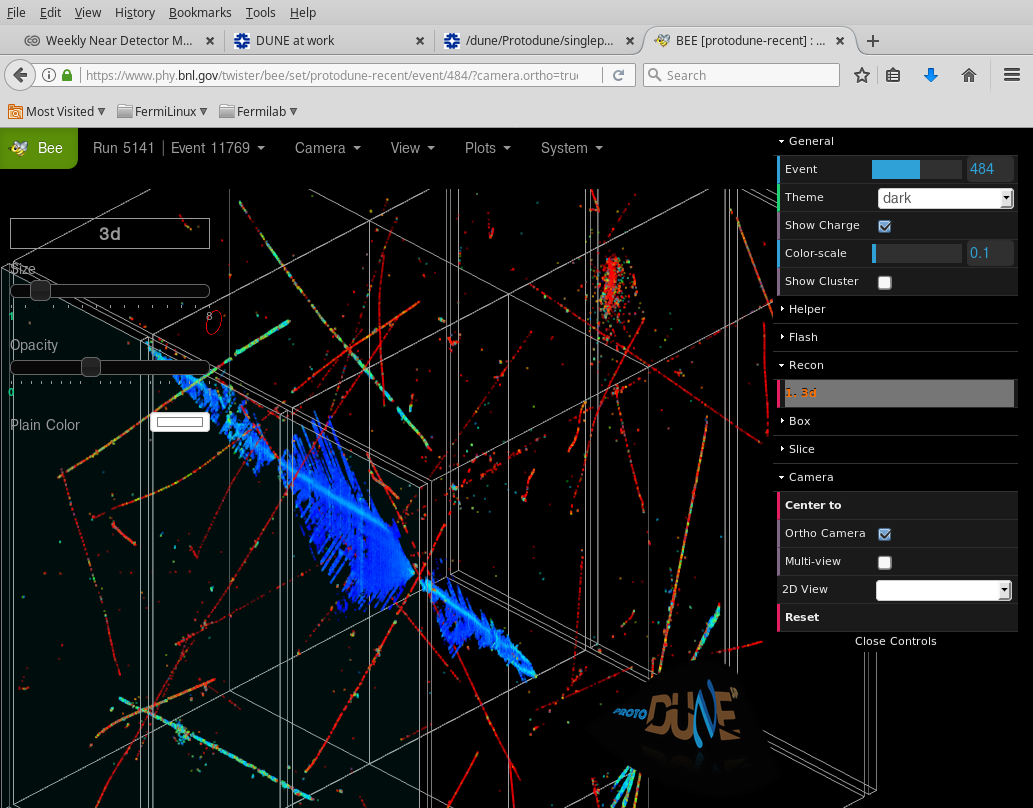
\includegraphics[width=0.9 \textwidth]{graphics/EventDisplays/bee_pdsp_evd1.png}
\end{dunefigure}

\todo{Can we get a bee with a white background? } 

Another web-based event display is called WebEVD.  It runs as a \dword{larsoft} module, and it sets up a local web server owned by the user process on an interactive computer.  The user then must ssh in to the interactive computer running the web server, with a specified port forwarded.  The user then connects to that port with a local web browser and interacts with the event display with it.  This user-owned web server which is only visible via authenticated ssh has the advantage that it provides the user with full control over which data are to be displayed, as the web server is not centrally managed.  An example display of two-dimensional deconvolved waveforms for a simulated $\nu_e$CC event in a \dword{fd} workspace geometry run is shown in Figure~\ref{fig:vis:webevd2d}.  An example three-dimensional event display from a \dword{pdsp} data run produce using WebEVD is shown in Figure~\ref{fig:vis:webevd3d}.

\begin{dunefigure}
[Two-dimensional WebEVD of a simulated $\nu_e$CC interaction.  ]
{fig:vis:webevd2d} 
{A simulated $\nu_e$CC interaction in a far detector workspace geometry run. The display is of charge reconstructed on collection wires (recob::Wire). The horizontal axis is the $z$-axis (beam direction) in the detector. The vertical axis corresponds to drift time ($x$ position in the detector). Both axes are labeled in cm. Rendered with WebEVD. }
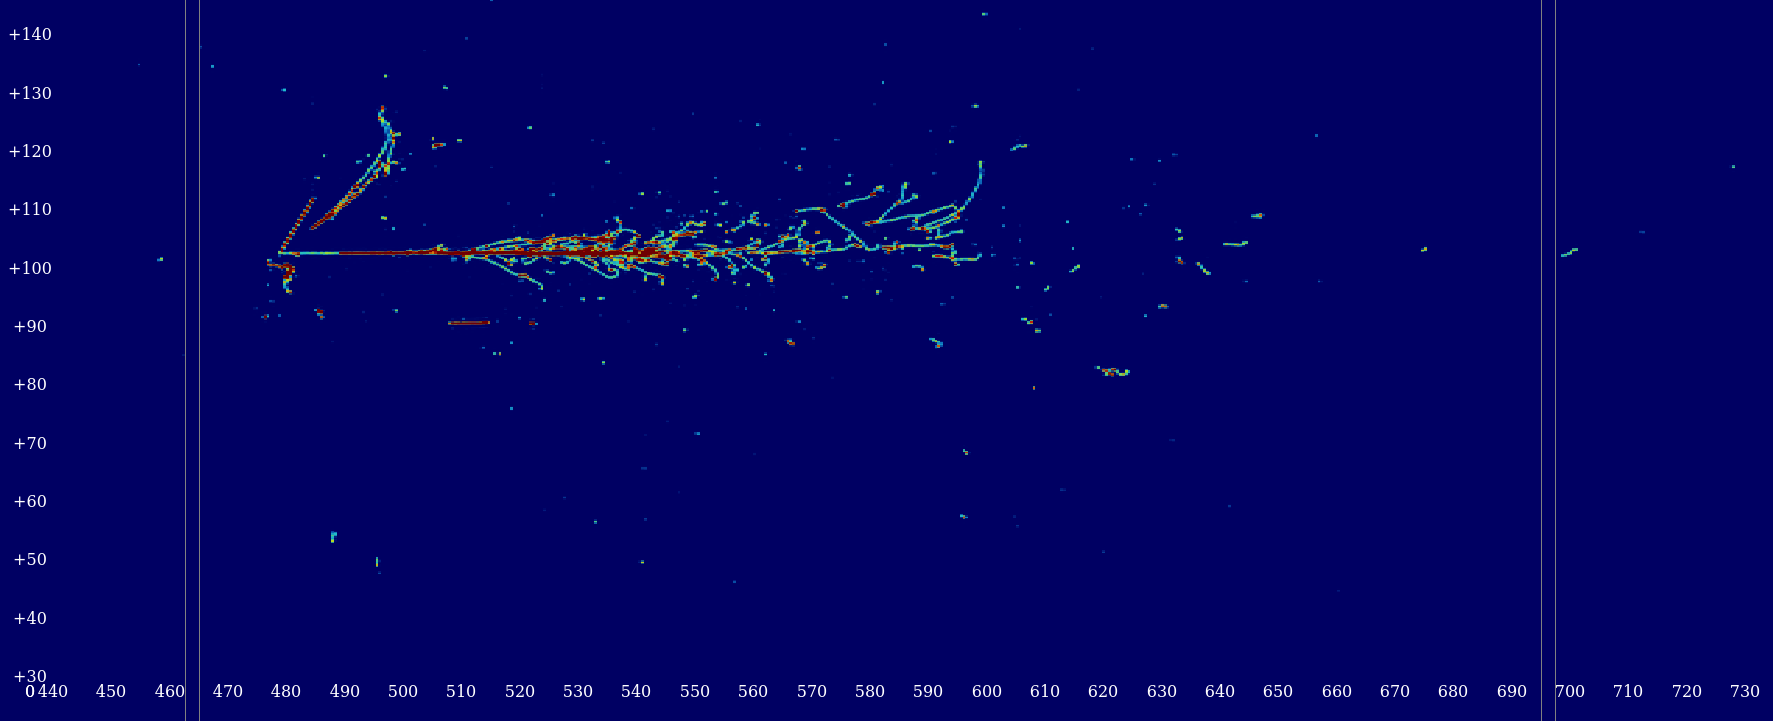
\includegraphics[width=0.9 \textwidth]{graphics/EventDisplays/webevd_nuecc_sim.png}
\end{dunefigure}

\begin{dunefigure}
[Three-dimensional WebEVD of a ProtoDUNE-SP trigger record. ]
{fig:vis:webevd3d} 
{ Example three-dimensional reconstructed data display for a \dword{pdsp} data trigger record, rendered with WebEVD. Reconstructed tracks and space points are shown in blue, and detector elements are shown in red.}
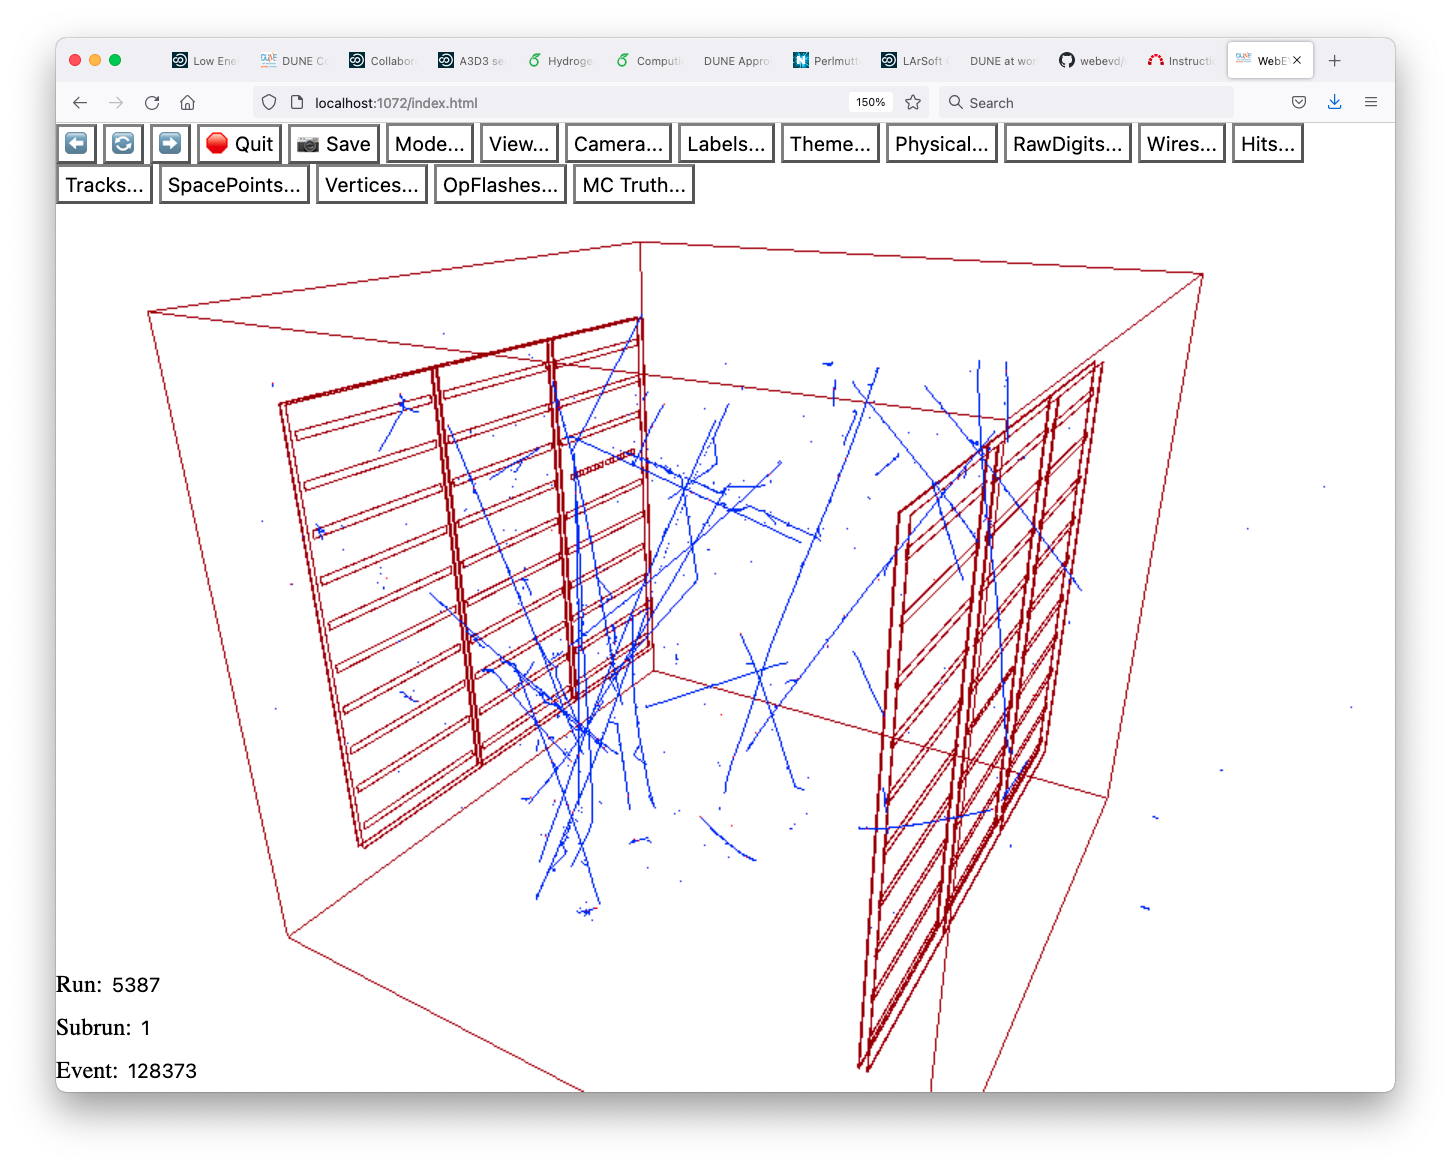
\includegraphics[width=0.9 \textwidth]{graphics/EventDisplays/webevd_pdsp3d.png}
\end{dunefigure}

\subsection{Near Detector Event Displays}
\label{sec:visualization:neardetector}

%TODO:  {\color{red}Add text and figure for ND-LAr.}

An example of a reconstructed event in \dword{ndgar} is shown in Figure~\ref{fig:vis:garsoftreco} rendered with the \dword{root}-based event display in \dword{garsoft}.  The same event is shown in Figure~\ref{fig:vis:garsoft2}, rendered with the TEve-based event display in \dword{garsoft}.

\begin{dunefigure}
[GArSoft reconstructed data display, ROOT-based]
{fig:vis:garsoftreco} 
{Example reconstructed $\nu_\mu$CC event produced with \dword{garsoft}, using an ALICE-inspired detector geometry.  The reconstructed vertex is indicated with a yellow dot, and tracks are shown in green, blue, and red.  Reconstructed calorimeter clusters are shown with green tetrahedra.  The annotations giving the \dword{mc} particle identities were added by hand.}
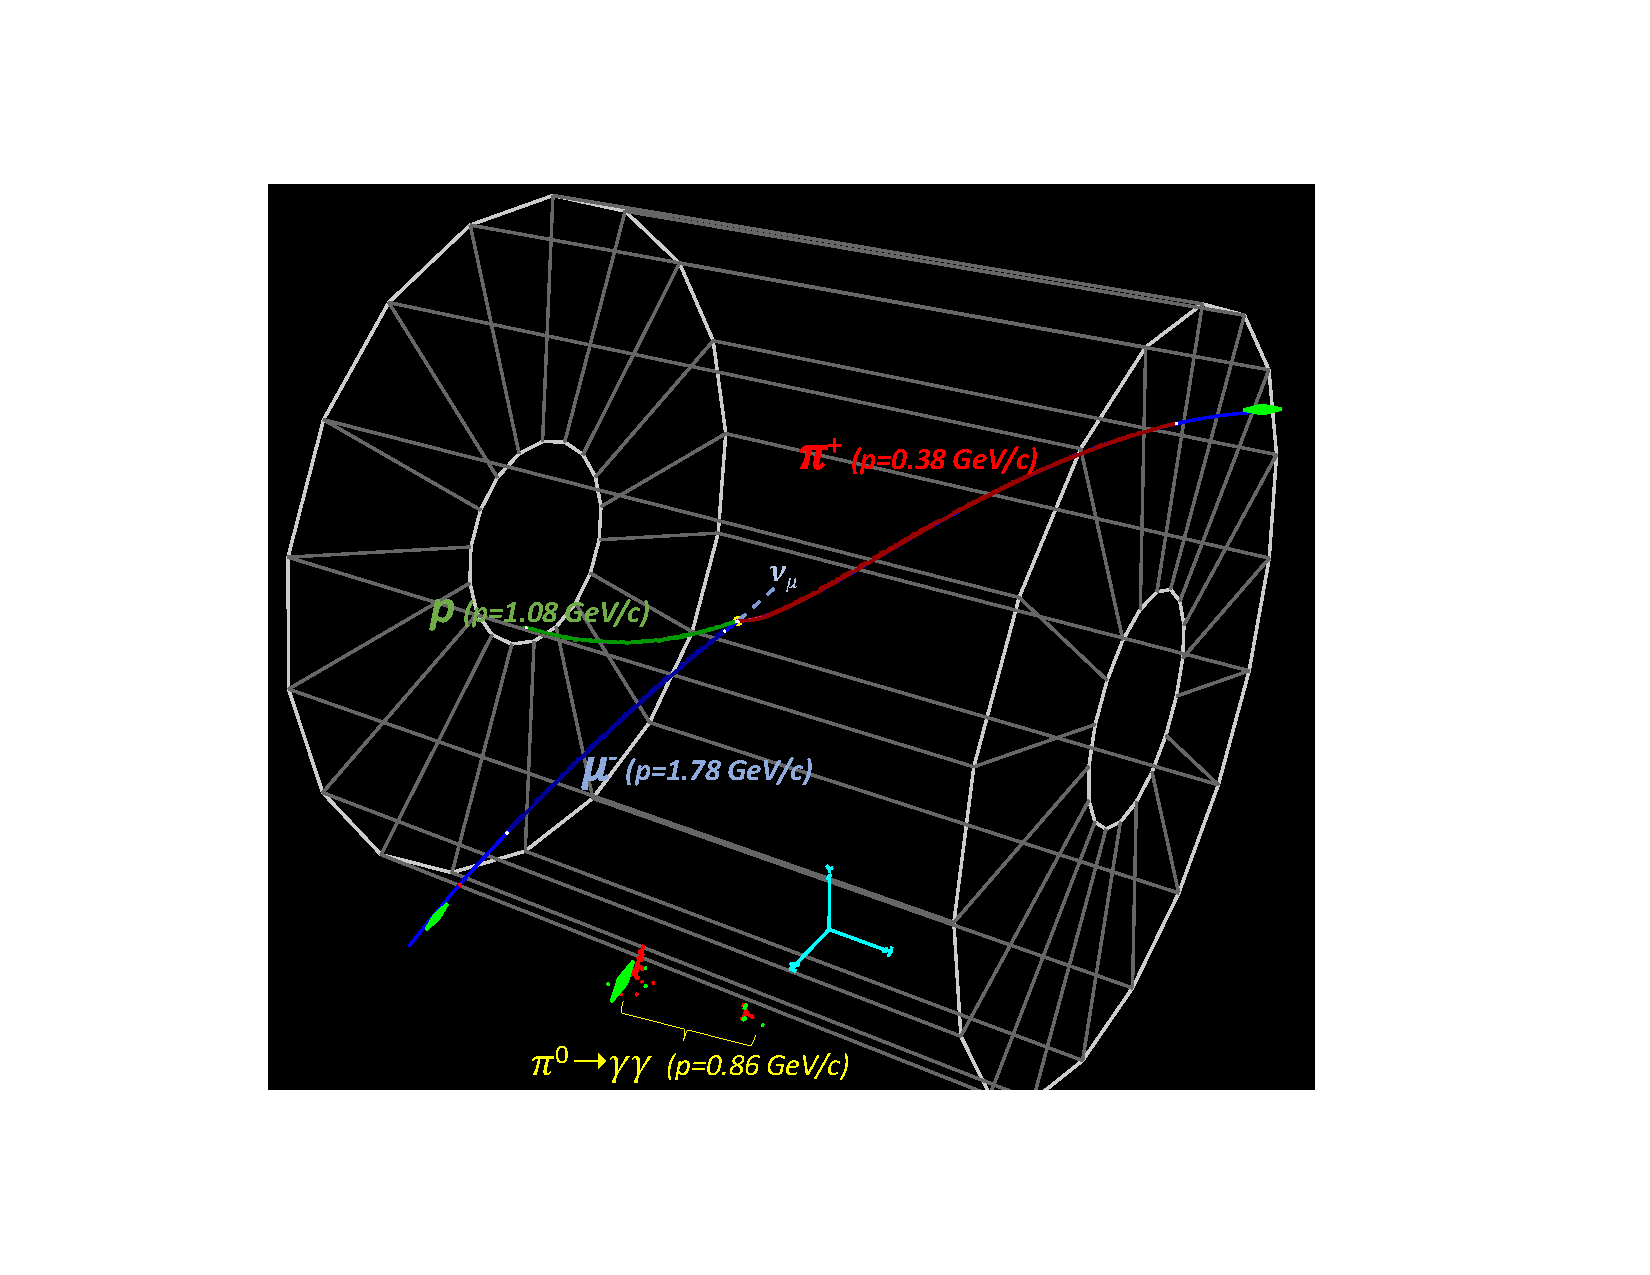
\includegraphics[width=0.9 \textwidth]{graphics/EventDisplays/nd_gar_evdwp2_withcaloclusters.pdf}
\end{dunefigure}

\begin{dunefigure}
[GArSoft Reconstructed data display, TEve-based]
{fig:vis:garsoft2} 
{The same \dword{ndgar} event as shown in Figure~\ref{fig:vis:garsoftreco}, rendered here with  \dword{garsoft}'s TEve-based event display.}
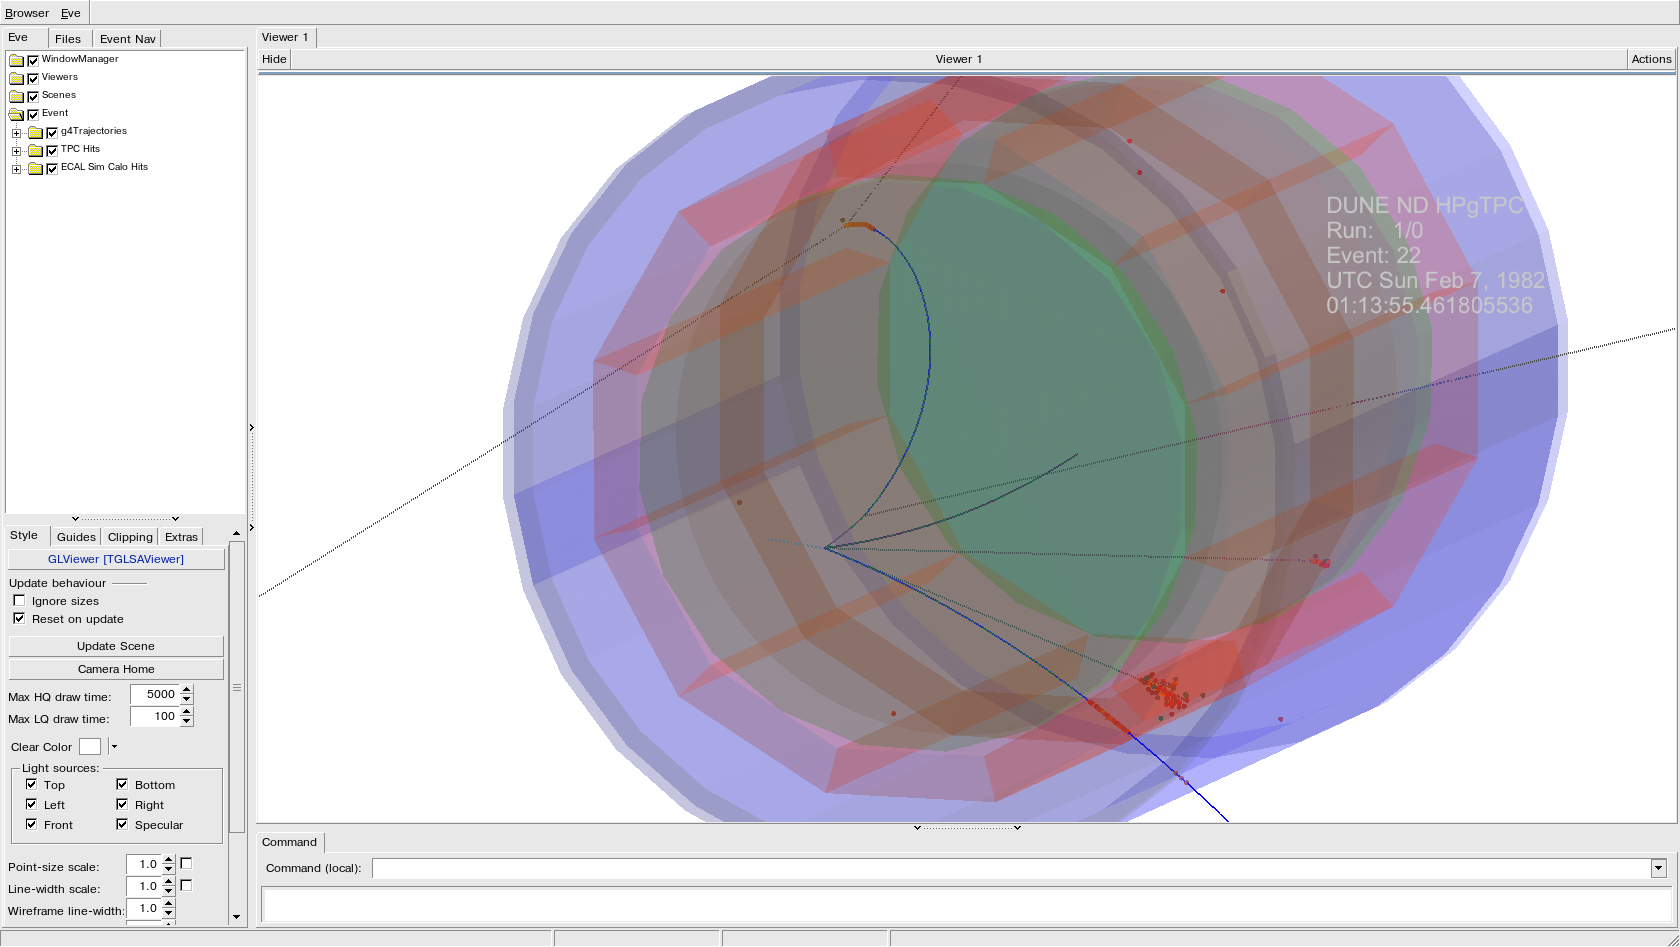
\includegraphics[width=0.9 \textwidth]{graphics/EventDisplays/ndgar_evd3d.png}
\end{dunefigure}

The third component of the near detector, \dword{sand}, consists of a staw-tube tracker and a calorimeter inside a solenoidal magnet.  A small cryostat containing liquid argon, called \dword{grain}, %anne 3/3: I added a dword; check def
is to be installed upstream of the straw-tube tracker inside the \dword{ecal}.  Design and performance studies are underway.  Basic event visualization tools have been developed to aid in the development of the reconstruction algorithms.  An example display of simulated and reconstructed particles in \dword{sand} is shown in Figure~\ref{fig:vis:sandevd}.

\begin{dunefigure}
[SAND Event Display]
{fig:vis:sandevd} 
{A rendering of a simulated full spill of neutrino interactions in the \dword{sand} detector. Magenta stars indicate true neutrino interaction vertices, blue curves indicate true simulated muon tracks, and thick green curves show proton tracks  Thin red lines indicate electrons and photons.  The red circles show the outline of the \dword{ecal}.  Blue dots indicate calorimeter hits.}
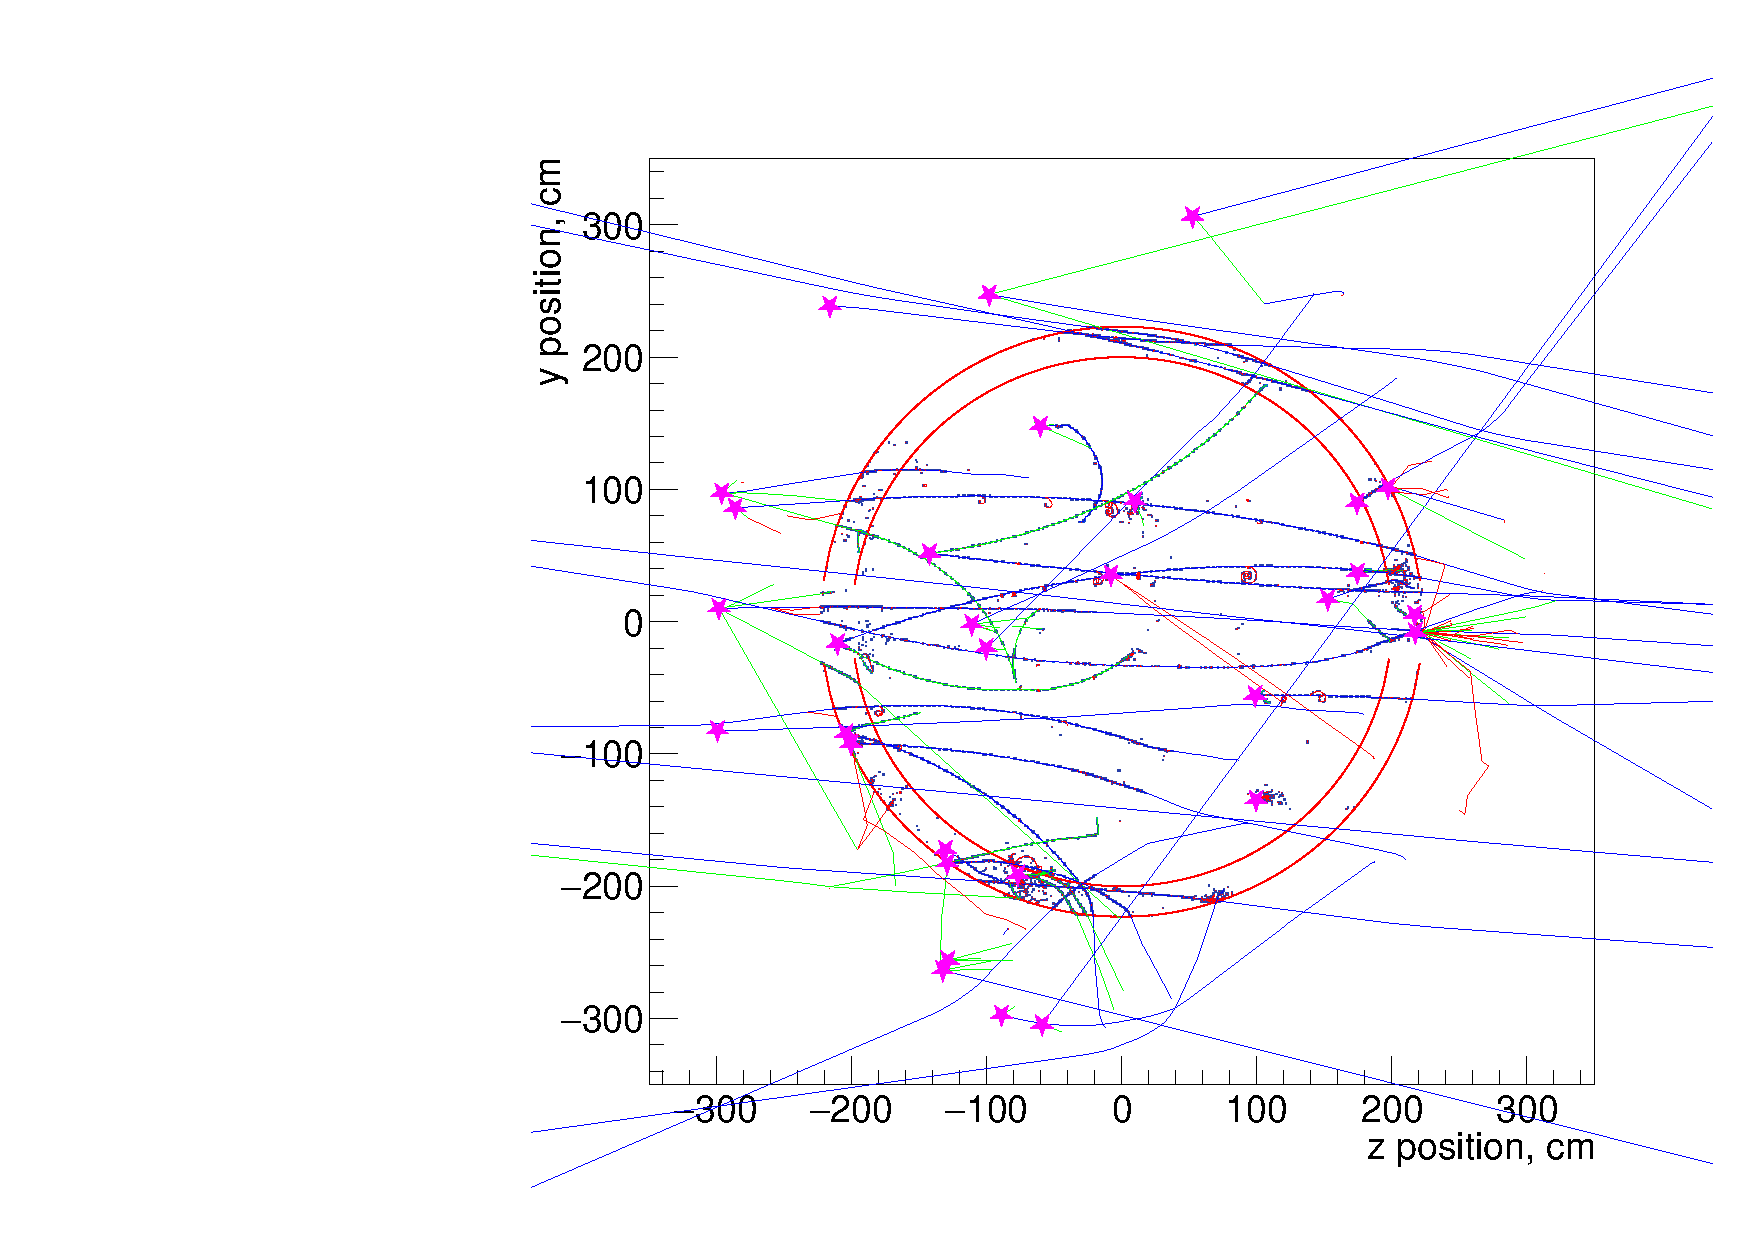
\includegraphics[width=0.9 \textwidth]{graphics/EventDisplays/sand_detector_view_stt_17924.pdf}
\end{dunefigure}

\section{Event Classification}
Events will need to be classified.  Much of this is now done using \dword{ml} techniques.  This can be done at any phase in processing from raw hits to the final stages of pattern recognition. Multiple groups are developing these algorithms and some are already part of the reconstruction chain.


\section{Analysis of Reduced Data Samples}
%\subsection{Production of Analysis Samples\hideme{Calcutt -NEW!!2/19}}

\subsection{Analysis Sample Production}
At some point in the processing, specialized datasets and streams based on trigger type, reconstructed event information, and intended use need to  be defined and produced.

The interaction data, which are in the output format supplied by the full reconstruction are then reduced and reconfigured into analysis formats for use by users. 
In the long run this processing will be done as coherent production steps but may also be done by small groups while the data formats and procedures are being developed.

DUNE's primary analysis framework for oscillation physics is currently the \dword{cafana} framework, originally developed for the NOvA experiment \cite{Backhouse:2015wlj,  bib:cafana}. The HighLAnd framework used by T2K is also used for some analyses. 





{\it Challenge:  This phase of processing is I/O limited and can put considerable strain on storage and network resources.  This and calibration drive the need to put most of the reconstructed data and simulation on disk at distributed sites as described in Part~\ref{part:model}.
A typical \dword{pdsp} data or simulation pass produces  10,000--100,000 2-8\,GB reconstructed files and  then produces much smaller tuple outputs for analysis.  These reduction jobs stream using \dword{xrootd} and are I/O bound. Preliminary monitoring studies indicate that average input rates of 5-30\,MB/sec per process can be achieved within a single site, with aggregate rates of several GB/sec across multiple processes. We are currently mining data access records to measure rates and reliability as a function of source and sink. }



\subsection{Reduced Analysis Samples}

\subsubsection{General Considerations for Analysis}
Reduced data analysis samples  are the samples users see and analyze when they are not developing new reconstruction  or calibration algorithms. 

Analysis samples should be useful and as small as possible.  Analysis codes should not need to read from the central databases but may need to access small local replicas. 

Data analysis may be done on local clusters, on collaboration grid facilities using shared data samples, or in dedicated analysis facilities that offer advanced access methods such as the Columnar Analysis framework \dword{caffea}.  %\fixme{Caffea... needs clarification (anne)} 
This phase of processing is typically very I/O bound and requires fast access to smaller data samples. 


An important question is what auxiliary information is needed and how it will be delivered. In particular, geometry and run-quality information are often needed in final analysis stages while direct access to detailed electronics calibrations is less often needed. 

\subsection{Current Practices}

A survey of data analysis users was done in February 2022.  Analyzers were contacted through the physics groups and analysis Slack channels.  We received 29 responses with users from institutions in eight countries dominated by the US(14) and UK(8). 
Responses were spread across multiple physics efforts: \dword{protodune}	(13),
Near Detector	(5),
Low Energy FD	(9),
High Energy FD	(7) and 
Calibration	(5).  



Figure \ref{fig:ch:use:survey} summarizes the results.  \dword{larsoft} is used by most users (presumably for small scale tests or tuple creation).  Users then rely on their own ROOT-based C++ or Python code for the final analysis steps.  A small number of users use shared analysis frameworks such as \dword{cafana}, \dword{nuisance} and \dword{highland}.  Jupyter notebooks are becoming popular. %\fixme{(anne) add refs and/or dwords}

Users analyze their reduced samples (which range in size between 5 GB and 10 TB) on the \dshort{fnal} interactive machines, via the grid batch systems and on local clusters and desktops. 


Although the physics groups tend to use the same technologies to analyze their data, the particular data content of their tuples differs.  Many users generate their own formats (at considerable expense in time and effort). Physics groups are beginning to move to common shared production as the content choices stabilize.  A single common format with common content is unlikely to emerge given the wide range of content different use cases (calibration, far detector low-energy signal, near detector, \dword{protodune} studies) that are already present.

The current goal for computing infrastructure is to support a wide range of formats and analysis strategies while encouraging shared, well-documented, cataloged samples. 

\begin{dunefigure}
[DUNE analysis code survey responses]
{fig:ch:use:survey}
 {User responses to the analysis survey. Panels show the data formats used, the analysis frameworks used, the locations where the jobs are run, and the locations where code is kept.}
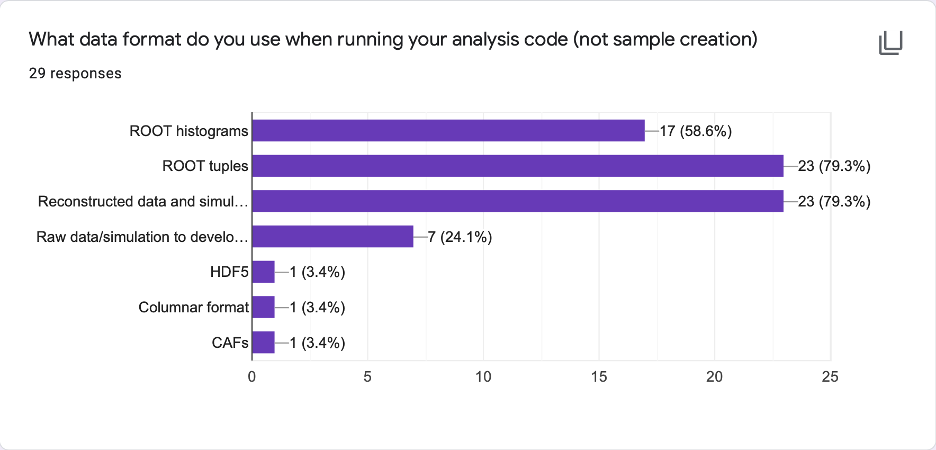
\includegraphics[width=6 in]{graphics/Algo/SurveyFormat.png}
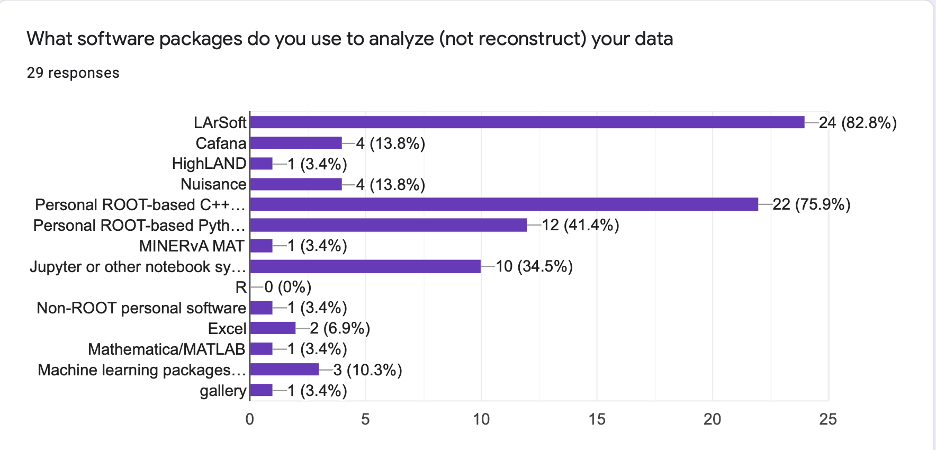
\includegraphics[width=6 in]{graphics/Algo/SurveyCode.png}
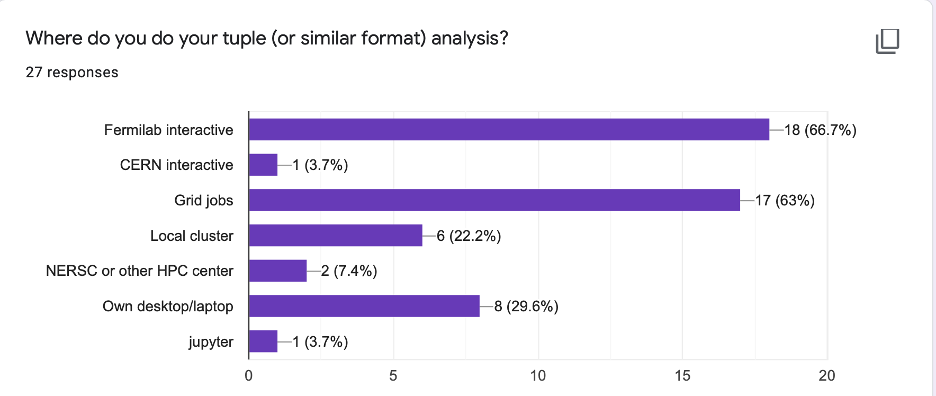
\includegraphics[width=6 in]{graphics/Algo/SurveySite.png}
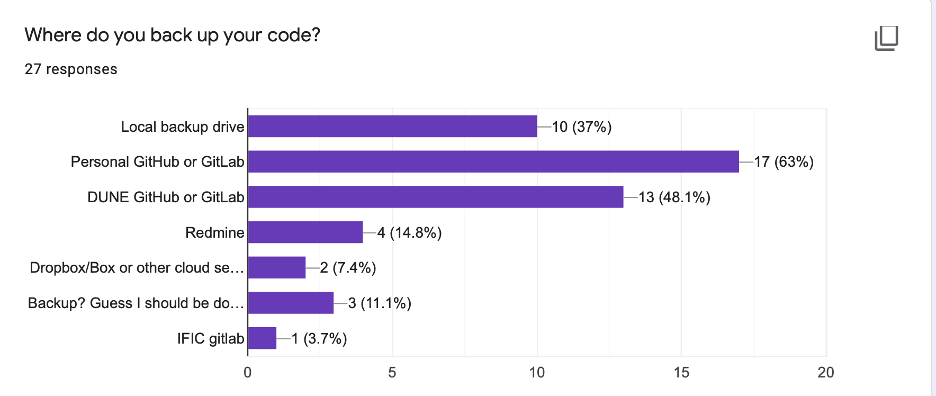
\includegraphics[width=6 in]{graphics/Algo/SurveyRepo.png}
\end{dunefigure}

\ignore{\subsection{Example of \dshort{protodune} Analysis \hideme{draft}}

\fixme{(anne) is this section really needed for a CDR? Lots of undefined terms and details, and the reader might get bogged down - I didn't review}

One of the \dword{protodune} analyzers %anne, Jacob Calcutt,  
provided information on workflow for a typical ongoing analysis. 


\subsubsection{Ntuple Production}

Standardized analysis ntuples are produced on the grid from the reconstructed PDSPProd4a simulation samples (133 TB, 691,200 events)  and  PDSPProd4 data (48 TB, 1,295,813 events )  for an example 1 GeV/c beam momentum setting. The tuple production code pdspana  partially reruns partial reconstruction to include updated calibrations and then extracts physics information and stores it in root ntuple format. The full MC ntuple took 2,332 CPU hours to create. The data ntuple took 335 CPU hours to create. This processing is found to be IO bound even when reading from local dCache storage at $\sim 20-30 $MB/s. The outputs are 14 and 13 GB in size respectively and cataloged in the \dword{sam} system.  

\subsubsection{Preliminary Event Selection Studies}

A set of python scripts are then used to produce distributions of important reconstructed observables. These are used to refine event selections, including determining cut values to use and estimating efficiencies and purities. These scripts use pyroot to interface with the data/mc files and to create/display the distributions. These studies  are done interactively on a dunegpvm virtual machine at Fermilab.
Refined ntuples are then produced with bad events (mainly those missing beam information) filtered out and labels applied to simulated information. The event selection code uses ROOT’s `RDataFrame' class to perform filtering and labeling. This takes about 20 minutes to perform for the full ntuples.  These final samples contain 159,083 data and 170,238 simulated events. 

\subsubsection{Cross Section Analysis Extraction}

The filtered/labeled ntuples are then passed to custom  ROOT based C++ fitting code for cross section extraction. Multiple types of extraction fits are performed with varying input parameters and samples, including data, full simulation and toy samples.  
Individual extractions are run interactively or on the grid for fake data tests and the ultimate real data fit. They can take O(5-45) minutes depending on how the fit is configured (i.e. what percentage of the input MC is used or how many parameter throws are performed post-fit to propagate error to measured/extracted cross sections). Sets of 1000 toy fits – where the nominal MC is systematically and statistically varied and used as fake data – are performed to study the overall behavior of a specific configuration of the fit.

}


%\section{Data Analysis on Reduced Samples \hideme{Schellman/David/Calcutt - needs work}}

%\todo{ - still on progress}

% Reduced data analysis samples  are the samples users see and analyze when they are not developing new reconstruction  or calibration algorithms. 

% Analysis samples should be useful and as small as possible.  Analysis codes should not need to read from the central databases but may access small local replicas. 

% Data analysis may be done on local clusters, on collaboration grid facilities using shared data samples or in dedicated analysis facilities that offer advanced access methods (Caffea ...). This phase of processing is typically very IO bound and requires fast access to smaller data samples. 


% An important question is what auxiliary information is needed and how it will be delivered. In particular, geometry and run quality information are often needed in final analysis stages while direct access to detailed electronics calibrations is less often needed. 
% \subsection{Current practices}

% A survey of data analysis users was done in February 2022.  Analyzers were contacted through the physics groups and analysis Slack Channels.  We receive 29 responses with users from institutions in eight countries dominated by the US(14) and UK(8). 
% Responses were spread across multiple physics efforts: ProtoDUNE	(13),
% Near Detector	(5),
% Low Energy FD	(9),
% High Energy FD	(7) and 
% Calibration	(5).  



% Figure \ref{fig:ch:use:survey} summarizes the results.  LArsoft is used by most users (presumably for small scale tests or tuple creation).  Users then rely on their own ROOT-based C++ or python code for the final analysis steps.  A small number of users use shared analysis frameworks such as cafana, Nuisance and HighLAND.  Jupyter notebooks are becoming popular. 

% Users analyze their reduced samples (which range in size between 5 GB and 10 TB) on the Fermilab interactive machines, via the grid batch systems and on local clusters and desktops. 


% Although the physics groups tend to use the same technologies to analyze their data the particular data content of their tuples differs.  Many users generate their own formats (at considerable expense in time and effort). Physics groups are beginning to move to common shared production as the content choices stabilize.  A single common format with common content is unlikely to emerge given the wide range of content different use cases (calibration, far detector low energy signal, near detector, protoDUNE studies) that are already present.

% The current goal for computing infrastructure is to support a wide range of formats and analysis strategies while encouraging shared, well-documented, cataloged samples. 

% \begin{dunefigure}
% [Dune code survey]
% {fig:ch:use:survey}
%  {User responses to the analysis survey. Panels show the data formats used, the analysis frameworks used, the locations where the jobs are run and the locations where code is kept.}
% 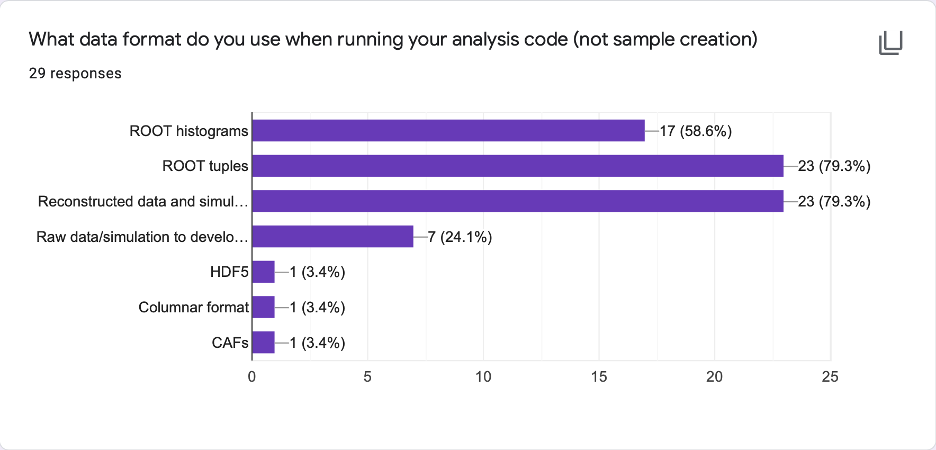
\includegraphics[width=4 in]{graphics/Algo/SurveyFormat.png}
% 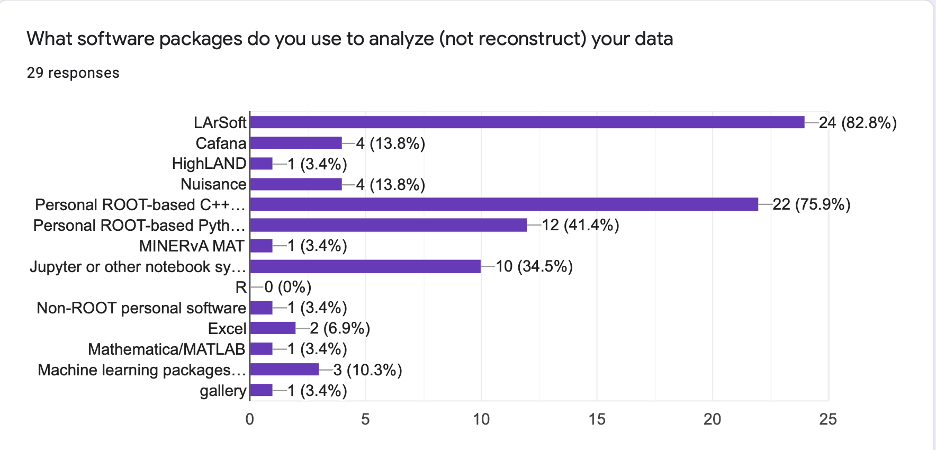
\includegraphics[width=4 in]{graphics/Algo/SurveyCode.png}
% 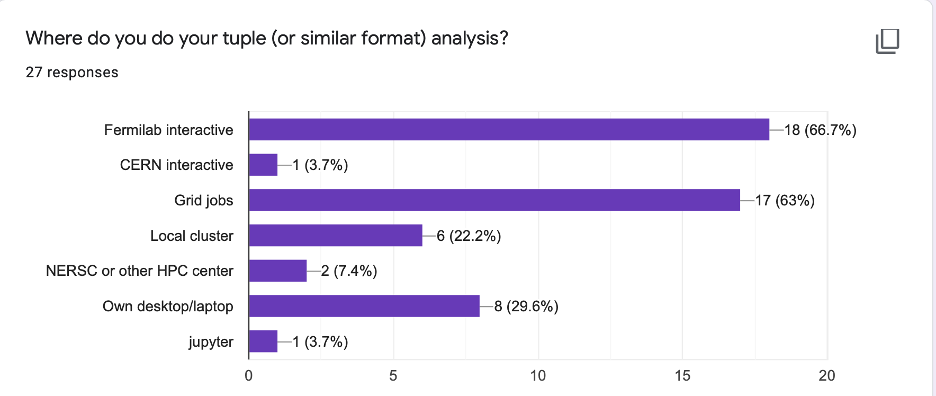
\includegraphics[width=4 in]{graphics/Algo/SurveySite.png}
% 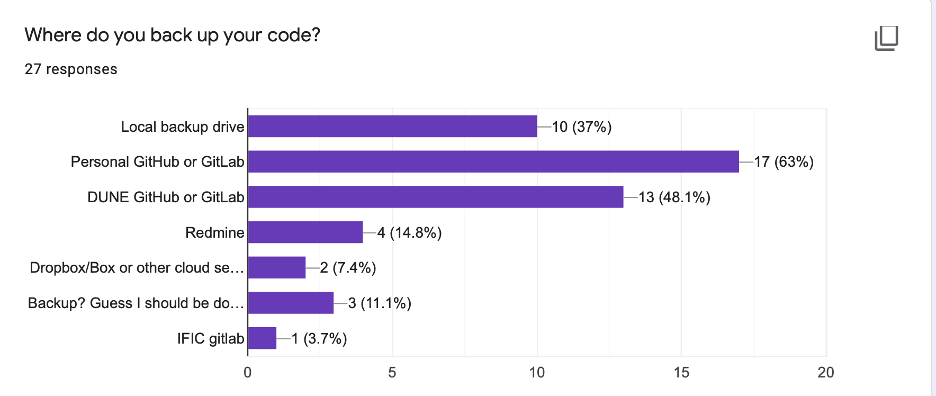
\includegraphics[width=4 in]{graphics/Algo/SurveyRepo.png}
% \end{dunefigure}
%\section{Other use cases}
\section{Machine Learning Training and Implementation} \hideme{HMS Updated to cite the Wang/Yang AWS paper}
Many reconstruction and simulation algorithms can profitably use \dword{ml} algorithms.  While these algorithms may run quickly, they   require significant resources to train, and in some cases, run much more efficiently on specialized hardware.  Although \dword{ml} algorithms are not currently a major part of the \dword{dune} workflow, multiple groups are working on implementing \dword{dune} algorithms on \dwords{gpu}.  A notable example is reference~\ref{Wang:2020fjr} in which \dword{protodune} reconstruction workflows on simulated far detector neutrino interactions are implemented via the \dword{sonic} framework developed at Fermilab. This hybrid framework enables the use of remote \dwords{gpu} as call-outs within the normal workflow.  In particular, the electromagnetic shower algorithm, {\it EmTrackMichelId}, which appears as the slowest algorithm in Table \ref{tab:protodune_cpu_reco_by_module} was implemented on commercial (Google Cloud) remote \dwords{gpu}. Patches of detector data were sent to the remote processors and inference results were returned.  In the initial test, event processing, which is dominated by that step, was sped up by a factor of 17. Similar approaches are very promising for the future.  


\section{Parameter Estimation}
Once final data samples are available, parameter estimation needs to be done to extract final oscillation and production  model parameters.  The NOvA oscillation parameter estimation \cite{NOvA:2021nfi} involved exploring of order 100 sources of uncertainty and was performed on the \dword{nersc} HPC systems.  

% \hideme{HMS suggest removing this as it just doesn't fit here anymore. \subsection{Database design and access}
% DUNE will need databases for a wide range of activities, from tracking detector construction to detailed calibration.  Chapter~\ref{ch:db} describes the database planning in detail.  Major considerations are the ability to  receive inputs from a wide variety of sources, some of which may have proprietary interfaces, and then to distribute information to a broad range of processing sites.   Use of open-source solutions is highly encouraged but may require additional effort.

% {\it The major challenge for DUNE, as for most database projects in the field, is the sheer amount of effort needed to carefully specify multiple problems and then deploy solutions that work at scale. As the database schema will be largely unique to DUNE, we can take advantage of existing general tools but much of the design must be closely tailored to our needs. The problem itself is not novel but the solution will require a large fraction of the total software effort.}
% }

\section{Summary: Characteristics of Large-Scale Processing Tasks}

A large number of complicated tasks have been listed above.  Table \ref{tab:tasks} summarizes the computing characteristics of the most prominent ones per MB of data. In combination with data volumes for any given task, these estimates can be used to predict processing needs as described in Chapter~\ref{ch:est} and to optimize data and job placement as described in Chapters~\ref{ch:datamgmt} and~\ref{ch:wkflow}. 

\begin{itemize}
    \item Simulation requires flux files (and possibly overlay libraries) as input but produces much larger outputs. The impact on networks is negligible but the memory needs are substantial.
    \item Reconstruction of data is assumed to be done by streaming from raw data, likely at a remote site. The processing time/MB is large enough that the impact on networks is minimal. 
    \item Ntuple creation and calibration require multiple passes over the reconstructed samples. Either local data stores or streaming from ``nearby'' sources is optimal as network speeds become important. Section~\ref{ch:model:perf} describes studies of job throughput as a function of disk and CPU locality. 
    \item Parameter estimation has been done using the \dword{hpc} resources at \dword{nersc}.  In this case a small amount of input data is processed simultaneously with systematic variations across a large number of cores. 

\end{itemize}

\begin{dunetable}
[Summary of computing resources needed per file]
{l r r r r r r }
{tab:tasks}
{Summary of resources needed per file for compute intensive tasks. The total CPU needed for a task can be determined from the total size of the sample and these numbers.}
Use case	&memory &	input file size &	output file size 	&	CPU time 	&	input  	& cores/job		\\
units	&GB	& MB	&MB	&	sec	& MB/s	&		\\

Simulation+reco	&		6	&	100	&	2000	&	27000	&	0.00	&	1	\\
data reco	&	4	&	8000	&	4000	&	60000	&	0.13	&	1		\\
tuple creation	&	3	&	4000	&	1	&	100	&	40.00	& 1		\\
calibration	&	3	&	4000	&	1	&	100	&	40.00	& 1		\\
%Parameter estimation	&		&		&		&		&		&			\\
\end{dunetable}
%\todo{Need Andrew N. or Norm N. to 

%\hideme{HMS eliminate this section and incorporate where relevant\section{Additional Activities}}% - \hideme{needs checking for completeness}}
\end{document}
